\chapter{\label{ch:1-intro}Introduction} 

\minitoc

\section{Setting the scene}

The costs of DNA sequencing have dropped significantly over the last couple of decades, from \$2.7 billion to sequence one human genome in the Human Genome Project \cite{Collins2003} to around \$600 \cite{Wetterstrand2022}. This dramatic reduction in cost has facilitated the generation of vast amounts of genetic data, enabling researchers to draw numerous inferences about the complexity of human genetics. With this influx of data, the field of statistical genetics has emerged as a critical area of study, focusing on the development of sophisticated statistical methods to manage and interpret this big data. Two main directions in statistical genetics deal with either learning about genetics forward in time or backward in time. Quantitative genetics looks forward in time and aims to understand how genetic variation affects observable phenotypes, providing valuable insights into the relationship between genes and traits. On the other hand, population genetics uses genomic data to look backward in time and aims to reconstruct the population history that has shaped present-day genetic diversity.

In this thesis, we leverage the massive amount of genomic data now available through rich datasets like the UK Biobank \cite{Bycroft2018}, the Human Genome Diversity Project \cite{Cann2002}, and the 1000 Genomes Project \cite{10002015} to explore both directions in statistical genetics. First, we look at population genetics, where we develop a method called GhostBuster to identify subtle differences in the genomic data and understand the evolutionary forces responsible for such changes. Second, we look at quantitative genetics, where we develop a method called Quickdraws to use the genetic variation data in present-day individuals for genome-wide association studies and to understand how this variation affects certain complex traits.

In this introductory chapter, we discuss the motivation, research aims, and literature review for analyses in Chapters 2 to 5. We structure the rest of the chapter to discuss the population genetics and quantitative genetics aspects separately. In Chapter 2, we introduce a novel method called GhostBuster, which relies on recent advances in building genome-wide genealogies at scale \cite{Speidel2019, Kelleher2019, zhang2023biobank}. In Chapter 3, we apply this method to understand the population structure in Africa. In Chapter 4, we shift to the quantitative genetics angle and introduce Quickdraws, a scalable variational inference method for performing genome-wide associations. In Chapter 5, we assess Quickdraws' efficiency, power, and robustness in simulations and real-data applications. Finally, in Chapter 6, we conclude our thesis by mentioning the key takeaways and future work.

\section{Understanding population history through genetic data}

The study of how evolutionary forces impact genetics, and therefore phenotypes, has been conducted for more than a century. Even with limited data, mathematicians have theorized frameworks to understand the relationship between evolutionary forces and present-day genetics. With the availability of genetic data, it is now well-known that evolutionary forces such as mutations, recombination, selection, and demographic changes like population structure and admixture have impacted our present-day genetic makeup. In this thesis, we focus on two such important forces that have shaped the genetics of present-day individuals: admixture and population structure. In this chapter, we will discuss various established theoretical foundations to understand population history through genetic data, particularly genome-wide genealogies, and their application to recently available genomic data.

\subsection{Basic definitions}

Deoxyribonucleic acid (DNA) encodes the hereditary information of an individual. It consists of four nucleotide bases: adenine (A), cytosine (C), guanine (G), and thymine (T). Adenine pairs with thymine, and cytosine pairs with guanine, forming base pairs. Each nucleotide also includes a sugar molecule and a phosphate group. DNA sequences are arranged in a double helix structure, which is tightly coiled around proteins called histones to form chromosomes. Humans are diploid organisms, meaning they have two copies of each chromosome, one inherited from each parent. The human genome is compacted into 23 pairs of chromosomes, of which 22 pairs are autosomal chromosomes shared by both sexes, while one pair is sex-specific. DNA varies between individuals due to evolutionary processes such as mutations and recombination.

Mutations are random errors that occur during the copying of genetic material, leading to changes in the DNA sequence. While mutations can occur in any cell, those occurring in germ cells are passed down to offspring and are called germline or de novo mutations. Humans have an estimated average mutation rate of $1.2 \times 10^{-8}$ per nucleotide per generation \cite{Kong2012}, with males contributing more de novo mutations than females \cite{Harris2019}. On average, humans carry 70 de novo mutations compared to their parents. These mutations can be of various types, including single nucleotide variants (SNVs), which are the most common and involve the alteration of a single nucleotide base. Insertions and deletions (indels) involve the addition or removal of one or more nucleotide bases, copy number variants (CNVs) result in the duplication or deletion of large DNA chapters, and structural variants encompass even larger DNA alterations.

Recombination is another vital mechanism that ensures genetic diversity in various eukaryotes. In humans, recombination occurs during meiosis, a type of cell division responsible for the production of germ cells. During meiosis, the chromosomes from each parent align and cross over, creating a mosaic of both parental chromosomes. Consequently, offspring inherit a proportion of their genetic material from maternal chromosomes and a portion from paternal chromosomes. In most mammals, including humans, the locations of these crossover events are concentrated in specific regions of the chromosomes called recombination hotspots. It has been shown that the location of these hotspots is determined by a crucial gene called PRDM9 \cite{Baudat2010}.

Apart from mutations and recombination, which are stochastic in nature, various demographic factors like population structure, migration and admixture also influence the genetic makeup of present-day individuals. Population structure is defined as a systematic difference in allele frequencies between subpopulations. This occurs due to non-random mating within a population, either due to geography or other factors. For example, the geographic distance between continents has caused human populations within a certain continent to mix more frequently among themselves than with populations from other continents, resulting in systematic genetic differences between individuals from different continents. It has also been shown recently that population structure within humans exists not only on a continental scale but also within smaller geographical regions, termed fine-scale population structure.

Another important demographic factor which influences the present-day genetics is migrations. It can be understood as systematic movement of genetic material from one population to another. With the availability of genetic data and archaeological records we have now established several migrations in the human history. For example it is now well established there was a huge wave of migration of anatomically modern humans from Africa to Eurasia around 50,000-100,000 years ago which gave rise to present-day non African populations. More recently, there have been migrations from East Asia to America \cite{reich2012reconstructing}, spread of Anatolian or farming ancestry in Europe \cite{lazaridis2014ancient} and a rapid migration from the steppe into Europe and south Asia \cite{haak2015massive}.

Migrations typically involve geographic movement of individuals over an extended duration of time, but two populations can mix more abruptly or over a shorter time duration. This is referred to as an admixture event. Admixture affects genetics by producing offspring that are a mixture of two or more distinct subpopulations. Some examples of previously documented admixtures in humans include present-day African American individuals in America, whose genomes are admixed from African, Native American, and European sources \cite{smith2004high, price2009sensitive}. Introgression is similar to admixture except it involves small amount of gene-flow from one population to another usually involving populations or species which are very diverged. For example, the Neanderthal introgression into humans, which has resulted in 1-3\% of modern day non African DNA to come from Neanderthals \cite{sankararaman2014genomic}. Similarly, Denisovan introgression into South Asia and Oceania, contributes upto 5\% of Denisovan ancestry in Papuans \cite{reich2010genetic}. 

When two subpopulations admix, we often don't know these source groups. It might also be possible that, due to extensive admixture, we no longer have source groups that are 100\% comprised of one subpopulation or another. We define ghost populations as populations that contributed their genetic material to present-day individuals but are no longer present in the genetic pool of modern-day samples. As these populations no longer exist or have not been sampled, the only way to identify ghost populations or events is by carefully analyzing patterns in present-day genetic variation data to infer if there are signatures of any population structure or admixture events in the past.

\subsection{Theoretical framework to understand population history from genetic data}

The Wright-Fisher model \cite{Wright1931, Fisher1930} is one of the most popular population genetics model which formalizes how populations trace their ancestry backward in time.  The Wright-Fisher model simulates the genetic history of samples as follows: (i) Starting with $N$ haploid individuals in the population, each individual, going backward in time, chooses its ancestor from a set of $N$ ancestors with replacement. (ii) Generations are discrete and do not overlap, so (i) can be repeated backward in time until there is only one common ancestor. Furthermore, the Wright-Fisher model assumes tracing a single-site, equality of fitness and lack of any population structure. A simple depiction of how the common ancestor is chosen backward in time for three lineages is shown in Figure \ref{fig:coalescent}.

\begin{figure}[h!]
    \centering
    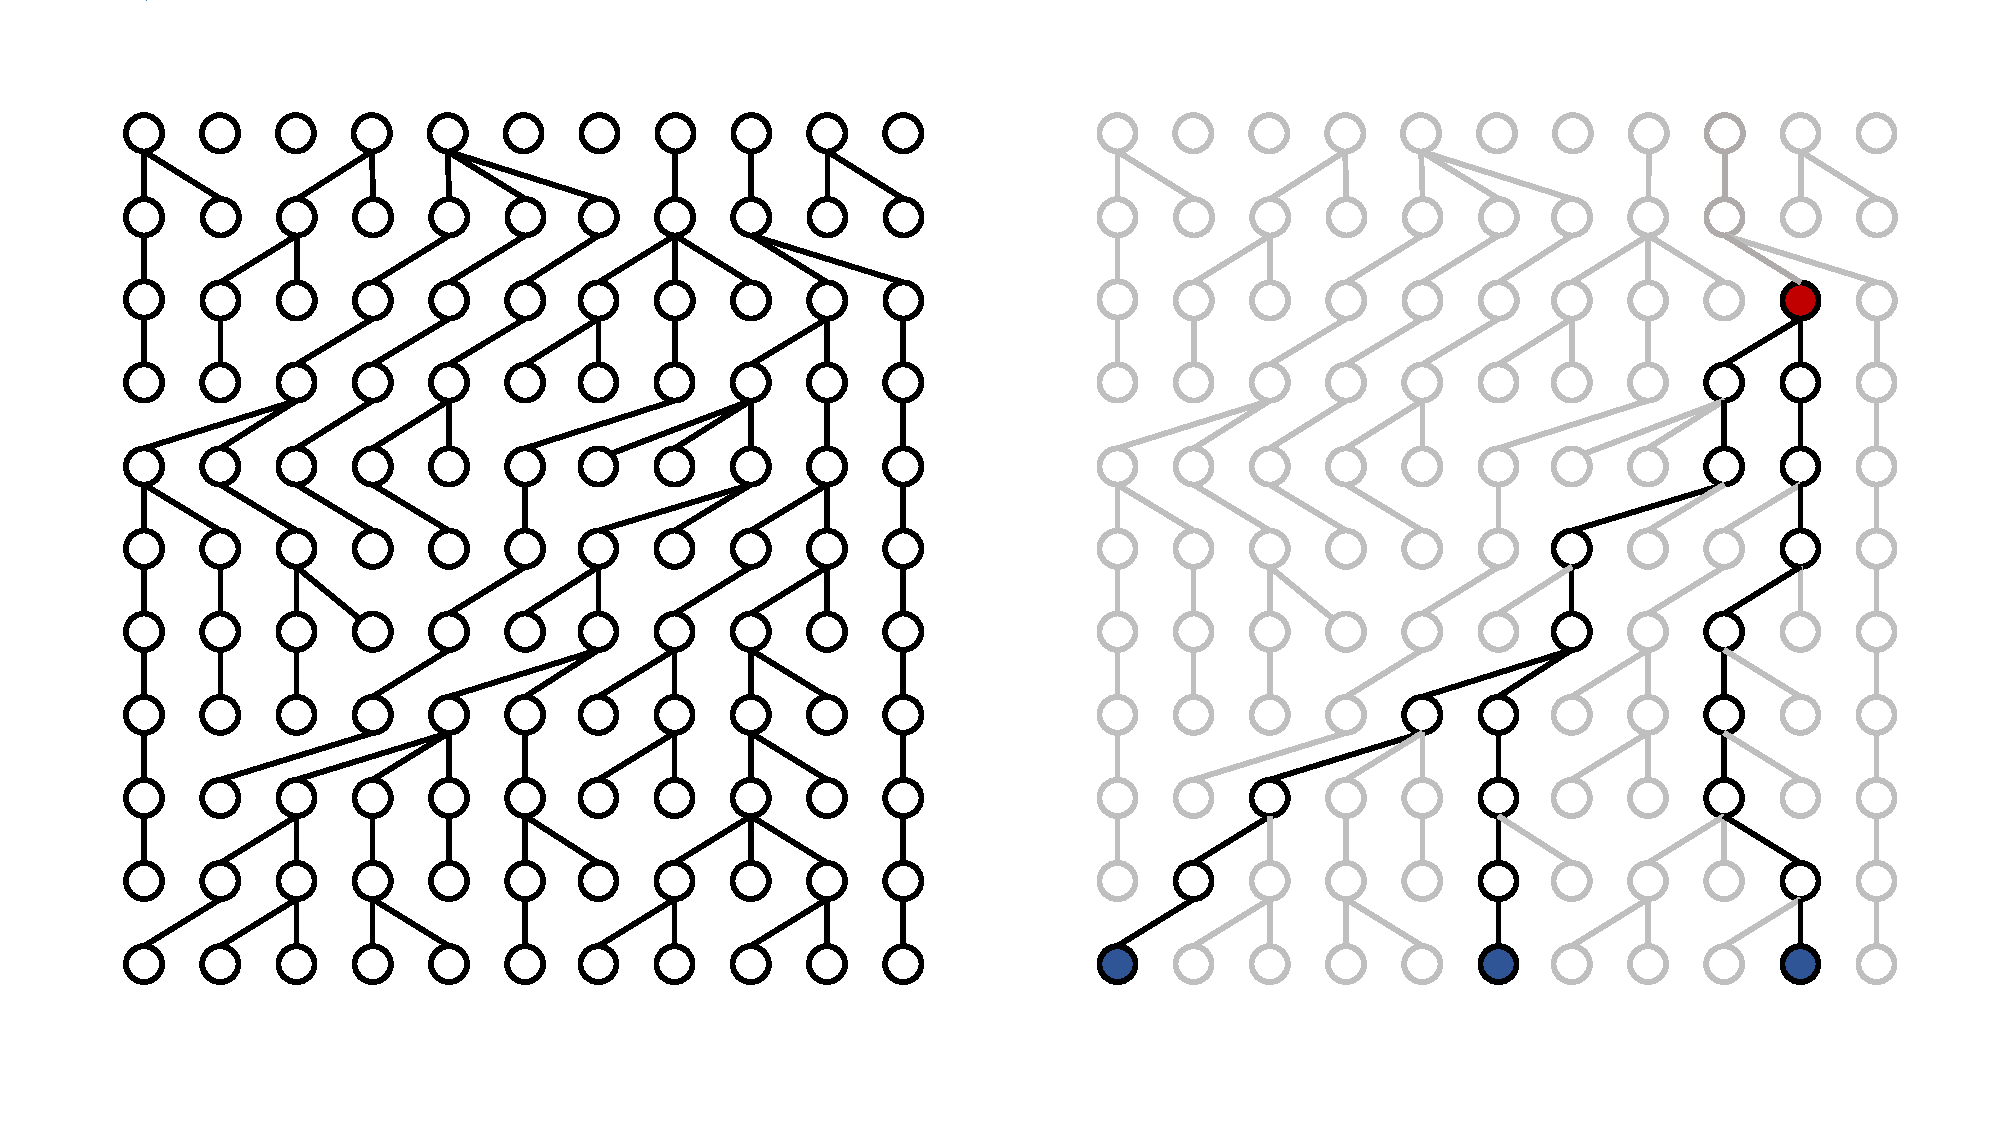
\includegraphics[width=\linewidth]{figures/wright_fisher.pdf}
    \caption{\textbf{Example of three lineages coalescing backwards in time in the Wright Fisher model.} Each individual chooses its ancestors from the set of ancestors with replacement until all the lineages coalesce into a single common ancestor. The three samples are coloured blue and the common ancestor for the three samples red }
    \label{fig:coalescent}
\end{figure}

Its possible to derive the probability distribution of the time to the most recent common ancestor (TMRCA) under the Wright-Fisher model assuming a constant effective population size $N_e$. The TMRCA for a pair of samples is geometrically distributed and takes the form:
\begin{equation}
P(\tau_2 = t) = \left(1 - \frac{1}{N_e}\right)^{\tau_2-1} \frac{1}{N_e}
\end{equation}

where $\tau_2$ is the time to most recent common ancestor, and $N_e$ is the effective population size. The cumulative distribution function (cdf) of $\tau_2$ looks like:
\begin{equation}
P(\tau_2 \leq t) = 1 - \left(1 - \frac{1}{N_e}\right)^{\tau_2}
\end{equation}

Assuming a large and constant population size, $N_e \rightarrow \infty$ and setting $T_2 = \frac{\tau_2}{N_e}$ we can approximate the cdf as follows:
\begin{equation}
\begin{aligned}
    P(T_2 \leq t) &= P(\tau_2 \leq N_et) = P(\tau_2 \leq \lfloor N_et \rfloor) \\
    &= 1 - \left(1 - \frac{1}{N_e}\right)^{\lfloor N_et \rfloor} \\
    & \rightarrow 1 - e^{-t} \text{  as  } N_e \rightarrow \infty
\end{aligned}
\end{equation}

Note that the TMRCA takes the form of a standard exponential distribution. This is the coalescent model, introduced by Kingman in 1982 \cite{Kingman1982, Kingman1982b, Kingman1982c}. As we will see the coalescent is a simplification of the Wright-Fisher model \cite{Wright1931, Fisher1930} for large populations which generalizes to various features in human genetics like mutations, recombinations and population structure. 

Its possible to generalize the coalescent to \(n\) lineages instead of a pair. Lets define $\xi(\tau)$ as the number of lineages remaining at time $\tau$. Going backward in time with the initialization $\xi(0) = n$, $\xi(\tau)$ behaves as a Markov process. That is the distribution of $\xi(\tau + 1)$ only depends on the previous one, $\xi(\tau)$. We can define the transition probability of going from $i$ lineages to $j$ lineages in one generation as:
\begin{equation}
    p_{i,j} = P(\xi(\tau + 1) = j \mid \xi(\tau) = i)
\end{equation}

It can be shown under the standard coalescent model, setting $N_e \rightarrow \infty$ and ignoring second order terms, the transition matrix simplifies as follows:
\begin{equation}
\begin{aligned}
    &p_{i,i} \approx 1 -  \frac{\binom{i}{2}}{N_e} \\
    &p_{i,i-1} \approx \frac{\binom{i}{2}}{N_e} \\
    &p_{i,j} \approx 0 \text{  for any  } j < i - 1
\end{aligned}
\end{equation}

Which implies the coalescent for \(n\) samples only allows one pair of lineages to coalesce per generation, making a binary ``coalescent'' tree. Additionally, the rate of coalescence depends on the number of lineages present at a given time. Let $T_j = \frac{\tau_j}{N_e}$ be the times when $j$ ancestors remain (scaled by the population size $N_e$) then according to the coalescent $T_j$ is independent of $T_i$ ($i \neq j$) and is distributed as follows:
\begin{equation}
    T_j \sim exp \left( \binom{j}{2} \right)  \text{,   } f_j(t) =  \binom{j}{2}e^{- \binom{j}{2}t}
\end{equation}

Its possible to generalize the above model for time-varying population sizes. Lets define the effective population size at time $t$ as $N_e(t)$. We can write the effective population size as a linear product of population size at $t=0$ and relative population size $\nu(t)$. Scaling the coalescence times based on population size at $t=0$, $N_e(0)$ the probability distribution when $j$ ancestors remain is given as follows:
\begin{equation}
    P(T_j > t \mid T_n + T_{n-1} + ... + T_{j+1} = s) = exp\left( - \binom{j}{2} \int_{s}^{s+t} \frac{1}{\nu(u)} du  \right)
\label{eq:coal_general}
\end{equation}

The above equation simplifies to the standard coalescent with constant population size if we set $\nu(t) = 1$. 

%% mention about inference of coalescene rates from a pair of lineages

\textbf{Coalescent with mutations:} To simulate mutations on the coalescent, we make an additional assumption called the infinite sites assumption. This assumption states that whenever a mutation occurs, it will always result in a new and unique mutated site, thereby disallowing any site from having more than one mutation. In humans, where the size of the genome is on the order of \(10^9\) bases and the mutation rate is on the order of \(10^{-8}\) per base per generation, it is realistic to assume that a mutation doesn't hit the same site more than once. Under the infinite sites assumption, we can model mutations as a homogeneous Poisson process on the coalescent. This means the total number of mutation events will follow a Poisson distribution with mean \(\mu t L\), where \(\mu\) is the mutation rate per base pair per generation, \(t\) is the time to the most recent common ancestor in generations, and \(L\) is the length of the genomic span being considered in base pairs. This is the generative model. During inference, where we already have information about mutations, we aim to reconstruct population characteristics backward in time.

\textbf{Coalescent with recombination:} Only modeling mutation isn't enough to infer human population characteristics; another important feature of human genetics is recombination. We can modify the coalescent model to account for recombination as follows: Each pair of lineages can not only coalesce but also undergo recombination events, which split the ancestry of a single lineage into two parts. Going backward in time, at each generation, each segment of DNA can trace its ancestry independently, potentially to different ancestors. This process creates a branching structure where different segments of an individual's genome may trace back to different ancestors, creating a more complex ancestral structure than simple coalescence. This model is called the coalescent with recombination \cite{Hudson1983}. This graph structure was first introduced in \cite{Griffiths1997}, and is called the ancestral recombination graph (ARG). An illustrative example of an ARG is depicted in Figure \ref{fig:arg}. ARGs can also be seen approximately as a sequence of trees. Genome-wide inference of ARGs is also referred to as genome-wide genealogies. In this thesis, we use the terms genealogies, tree sequences, and ARGs interchangeably, but a more descriptive difference can be found in \cite{wong2023general}.

%% change this to ARGs = tree sequences
\begin{figure}[h!]
    \centering
    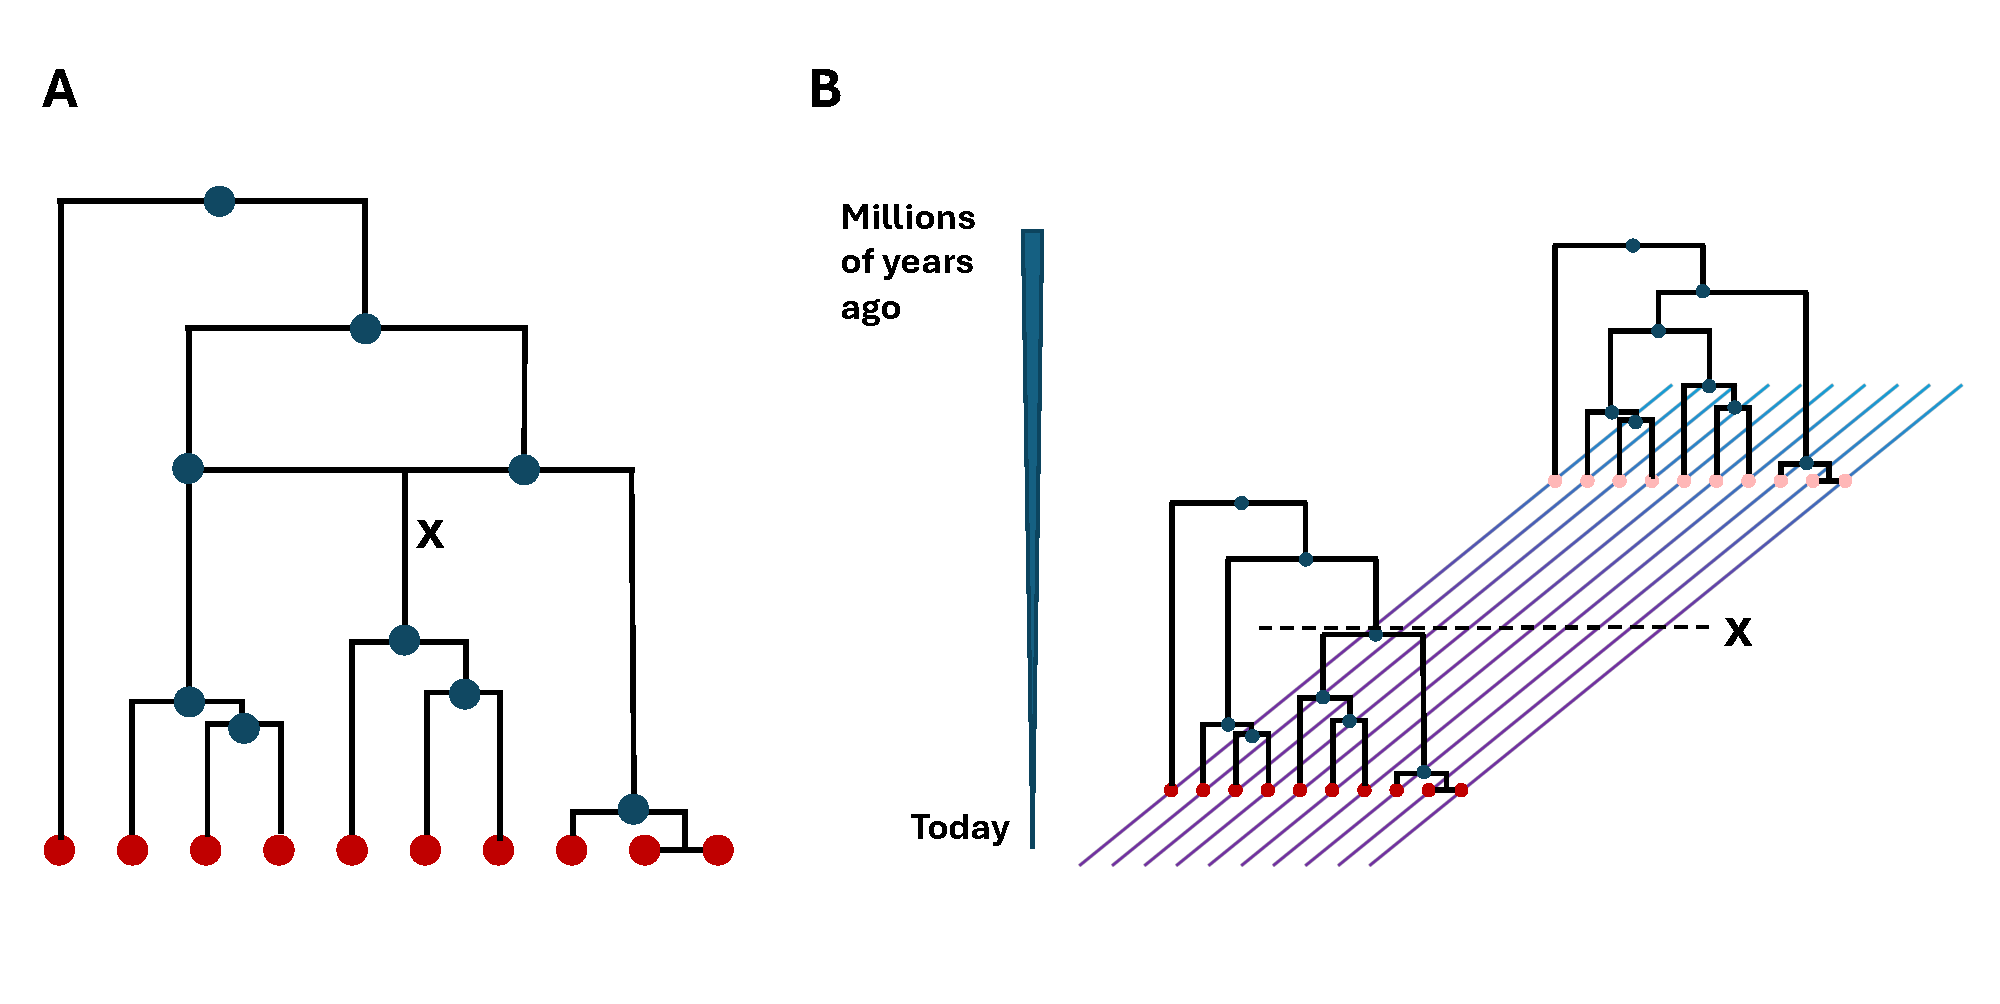
\includegraphics[width=\linewidth]{figures/coalescent_arg.pdf}
    \caption{\textbf{Example of an ancestral recombination graph (ARG) and the corresponding tree sequence.} (A) In the coalescent with recombination model the Lineages going backward in time can either coalesce or recombine, which means different portions of the genome have slightly different history. (B) Corresponding tree sequence representation of the ARG, \textbf{x} denotes the recombination site.}
    \label{fig:arg}
\end{figure}

The simplicity of the coalescent enables extending it to account for non-uniform recombination rates, time-varying population sizes and multiple samples. There is a suite of methods to infer these ARGs which rely on the coalescent theory. We will talk about these methods in chapter 1.2.4.

\textbf{Estimation of coalescence rates for a pair of lineages:} We can also perform inference under the coalescent. Lets simplify the coalescent for a pair of haplotypes and infer time-varying coalescence rates assuming piece-wise constant coalescence rates. We assume step-wise constant coalescence rates defined by fixed time intervals or epochs, labeled as $T_{e_1}$,  $T_{e_2}$, ... $T_{e_m}$. Lets say the coalescence rate is the parameter to be inferred and is given by $\gamma(e)$. The epoch index when the coalescence happens in the $l^{th}$ tree is given by $e_l$ and  the coalescence time is denoted by $t_l$ ($T_{e_l} \leq t_l \leq T_{e_l + 1} $). Extending the coalescent from equation \ref{eq:coal_general} for piece-wise constant coalescence rates, we can write the likelihood of the coalescence time as:

\begin{equation}
    P(t_l) = \gamma(e_l) e^{  -\gamma(e_l) (t_l - T_{e_l}) } \prod_{k=1}^{e_l} e ^{  -\gamma(e_l - 1) (T_{e_l} - T_{e_l-1}) } 
\end{equation}

For maximum likelihood estimation we assume the $T$ trees are independent so we sum the log-likelihood across trees and estimate the coalescence rates by maximizing the following:
\begin{align}
    \log P(t_l) &= \log \gamma(e_l)  -\gamma(e_l) (t_l - T_{e_l}) - \sum_{k=1}^{e_l} \gamma(e_l - 1) (T_{e_l} - T_{e_l-1}) \nonumber \\
    \log P(t) &= \sum_{l=1}^{T} \left( \log \gamma(e_l)  -\gamma(e_l) (t_l - T_{e_l}) - \sum_{k=1}^{e_l} \gamma(e_l - 1) (T_{e_l} - T_{e_l-1}) \right)
\end{align}

The MLE estimate for the coalescence rates are given by: 
\begin{equation}
    \hat{\gamma}(e) = \frac{n_e}{\sum_{l:e=e_l} (t_l - T_e) +  \sum_{l:e<e_l} (T_e - T_{e-1})}
\end{equation}

where, $n_e$ is the number of trees which coalesce in the $e^{th}$ epoch and is referred to as 'coalescence count' and $\sum_{l:e=e_l} (t_l - T_e) +  \sum_{l:e<e_l} (T_e - T_{e-1})$ is the sum of branch length until the haplotype coalesces and is referred as the `opportunity'. 

\subsection{Survey of methods to infer population structure and admixture history}
\label{sec:ch1-gb-survey}
Current methods to infer population structure can be classified into two main categories. The first set of approaches are called model-based approaches, where the methods rely on a predefined generative model of how the population structure would impact the genetics and use this model to solve the reverse problem of inferring the population structure given the genetics. Popular model-based methods to identify population structure include Structure \cite{Pritchard2000}, Admixture \cite{Alexander2009}, and FineStructure \cite{Lawson2012}. The other category of methods are non-model-based approaches, which don't rely on modeling assumptions and are more explorative in nature. Dimensionality reduction methods like principal component analysis (PCA) are a popular example of such methods. The choice of which method to use depends on the type of genetic data being analyzed, computational resources, data sizes, and modeling assumptions.

One of the earliest methods to understand population structure relied on quantifying genetic distances between individuals within and across pre-defined reference populations. One such measure, the `fixation index' also referred to as \(F_{st}\) \cite{Wright1951, Malecot1948}, measures the normalized allele frequency difference between two populations and within a population. Under several simplifying assumptions, including constant population sizes, the fixation index equals \(1 - T_0/T\), where \(T_0\) and \(T\) are the average coalescence times for individuals within the population and between two populations, respectively. The index is bounded from 0 to 1, where 0 refers to when the two populations are indistinguishable from each other, and 1 refers to when they are highly diverged. Since \(F_{st}\) measures genetic differences between populations due to genetic drift, population size plays a vital role in dictating how much drift is present. Smaller population sizes experience stronger drift, making methods that rely solely on \(F_{st}\) sensitive to assumptions about population sizes.

Early work to infer population structure also relied on analyzing variation in the Y-chromosome and mitochondrial DNA (mtDNA), as they have lost their ability to recombine \cite{Cann1987, tilford2001physical}. This allows for inferring a single genealogical tree that relates various populations, instead of an ARG or an average genealogical tree. In particular, the analysis of population structure using Y-chromosome or mitochondrial DNA involves considering prespecified `haplogroups', which are specific haplotypes thought to have arisen early in human history and are present in differing amounts in various human populations. By analyzing the number of specific haplogroups among populations, one can infer the coalescence times and topology of the genealogical tree explaining this pattern. Additionally, because Y-chromosomes are only inherited from the paternal lineage and mtDNA from the maternal lineage, this allows inference of population history that might be sex-biased. Although its importance in identifying sex-biased population structure persists even today, the number of haplogroups is limited, making it not always possible to discern subtle differences in populations by only looking at the Y-chromosome or mtDNA.

A popular model-based method to infer population structure is `STRUCTURE' \cite{Pritchard2000}, which clusters individuals into a fixed number of distinct populations based on their genotypic similarity. STRUCTURE assumes a similar generative model as latent Dirichlet allocation (LDA) in machine learning \cite{Blei2003}, which is used for topic modeling (though STRUCTURE predates LDA). The method works by partitioning the individuals into \(K\) populations, each characterized by allele frequency spectrum. It explicitly models the probability of observing the genotypes given the data and the assignment of the individual and proceeds with a Bayesian algorithm to infer the assignment of the individual and the corresponding allele frequencies that define the clusters. Several developments have improved the scalability of STRUCTURE, including methods like ADMIXTURE \cite{Alexander2009} and fastSTRUCTURE \cite{Raj2014}.

% cite eigenstrat
Principal component analysis (PCA) is a non-model-based method to infer and visualize population structure in the data \cite{menozzi1978synthetic,Patterson2006, Price2006}. It proceeds by eigen-decomposing the genotype matrix for all individuals and projecting the samples onto the top \(K\) eigenvectors. Due to eigen-decomposition, the top \(K\) eigenvectors maximize the amount of variance explained while being orthogonal to each other. It has been demonstrated that the top eigenvectors or principal components of the genotype matrix can capture the demographic history of samples without any specific modeling assumptions about the demography \cite{Patterson2006,novembre2008interpreting}. For example, the first two principal components (PCs) of a widely studied human genetic dataset, HGDP+1000 Genomes, clearly separate populations from sub-Saharan Africa from the rest of the samples. Furthermore, PC3 and PC4 start separating populations outside Africa. An accompanying plot which includes the principal components for the UK Biobank data is presented in Figure \ref{fig:pc_plot}. This plot is taken from \cite{Bycroft2018}.

\begin{figure}[h!]
    \centering
    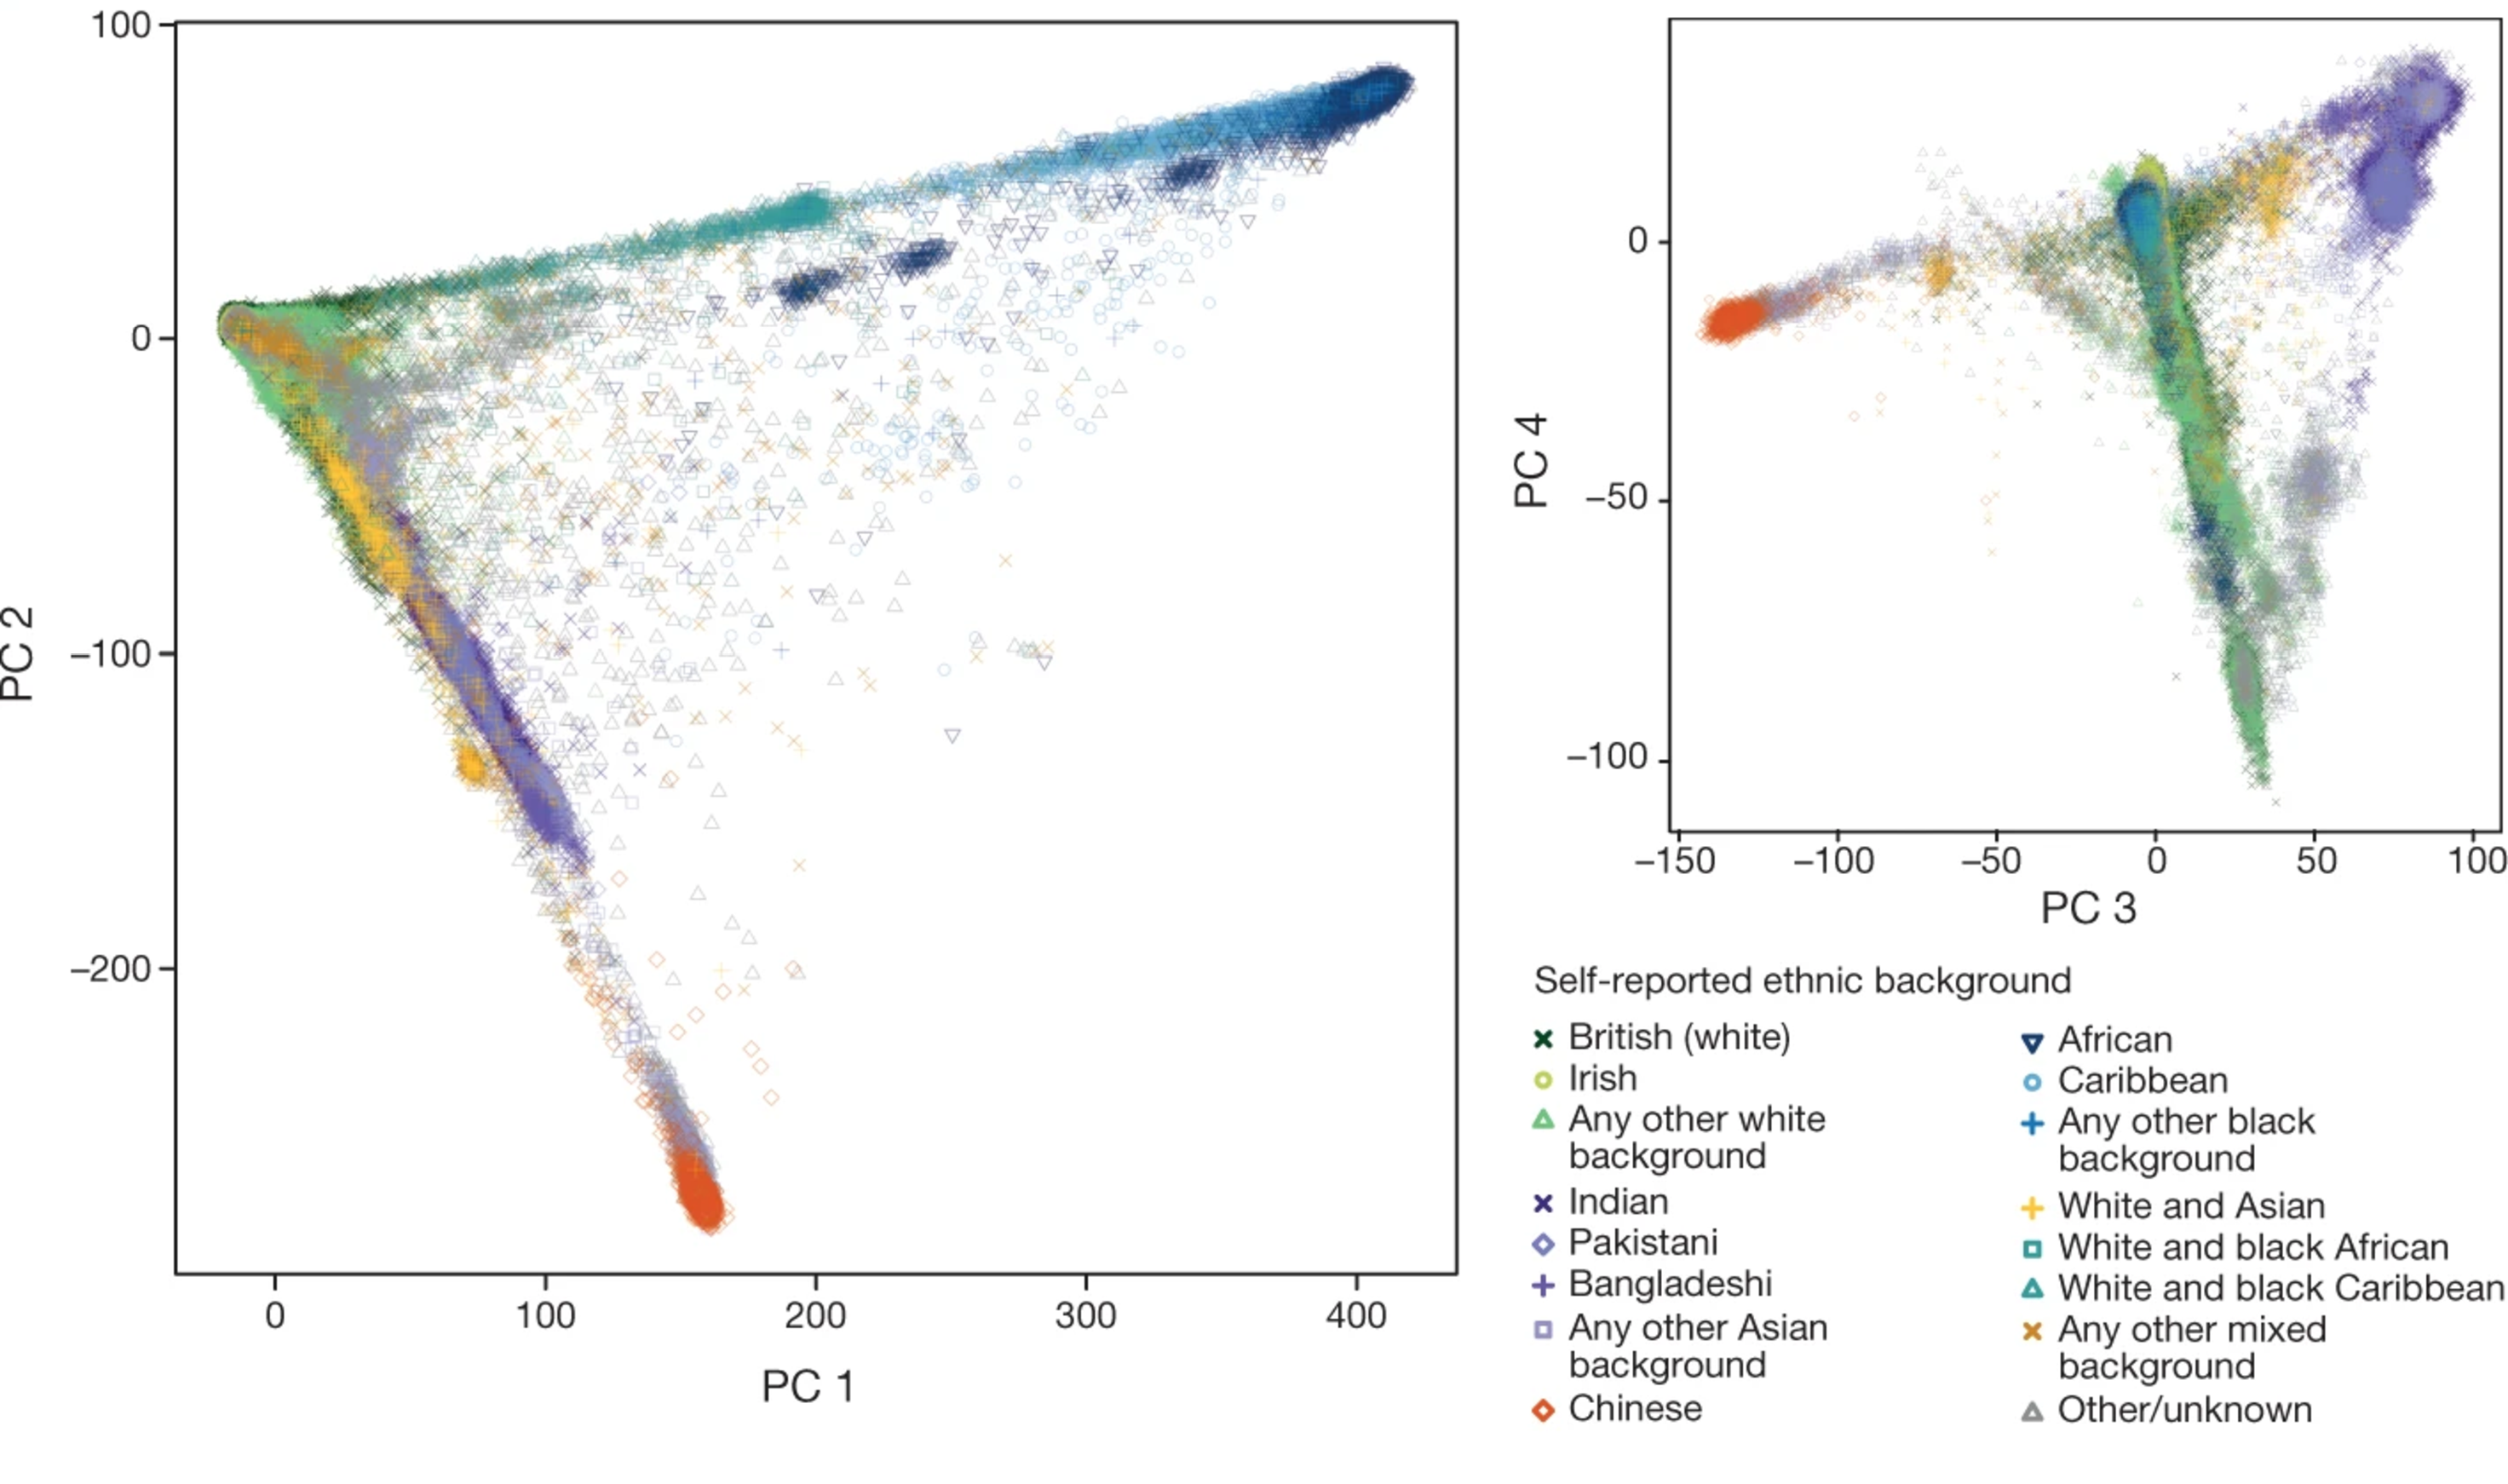
\includegraphics[width=\linewidth]{figures/thesis_pc_plot.pdf}
    \caption{\textbf{PCA visualization of $500,000$ individual genotypes from the UK Biobank.} PC1 and PC2 separates the African individuals from non-African individuals, whereas PC3 and PC4 separates individuals in Eurasia. The figure was taken from \cite{Bycroft2018}.}
    \label{fig:pc_plot}
\end{figure}

% cite plos one paper nick patterson
Both STRUCTURE and PCA work well when the population structure is strong, making differences in allele frequencies or genotypes among individuals identifiable from noise \cite{Patterson2006}. For more subtle differences in population structure, also referred to as fine-scale population structure, there are a suite of methods that rely on high-quality whole-genome sequencing data. Methods like ChromoPainter and FineStructure \cite{Lawson2012} are haplotype-based methods, which rely on high-coverage phased genotypes to infer more subtle population structure. Like STRUCTURE, ChromoPainter is also model-based, as it uses the Li and Stephens \cite{Li2003} algorithm to model an individual's haplotype as a mosaic of other individuals in a reference panel. Once the chromosome is painted, follow-up methods like FineStructure summarize the painting. The Li and Stephens algorithm is also used extensively to infer genealogies from sequencing data, as we will see in chapter 1.2.4.

Methods to identify population structure can also identify signatures of admixture in the data. For example, if there is recent admixture between two populations, the individuals who are admixed would have their STRUCTURE assignment as a mixture of two or more clusters, or would show a `cline' in the PCA, representing a continuum of ancestry between source groups. The American individuals in the HGDP+1000G dataset are admixed with varying admixture proportions from Native Americans, Europeans, and Africans, and this can be visualized in the PC plots in Figure \ref{fig:pc_plot}.

Other methods to infer admixture can characterize the admixture event more accurately. Methods like Globetrotter \cite{hellenthal2014genetic}, ALDER \cite{loh2013inferring}, and Rolloff \cite{moorjani2011history, patterson2012ancient} use haplotype information to infer admixture proportions, sources, and even admixture times. The idea behind these methods is based on the observation that if admixture is recent, there will be long segments of DNA from each ancestry because there has been less time for recombination to mix the ancestries thoroughly. In a simple 2-way admixture, the length of the DNA segment from a particular ancestry is exponentially distributed with the rate proportional to the admixture time; this is called a co-ancestry curve. More formally, the probability of no recombination between two points a distance g (in genetic distance units) apart since admixture is $e^{-g\lambda}$, where $\lambda$ is the admixture time. For a 2-way admixture, conditioning on recombination the joint probability of ancestries at a distance g apart is given as follows:

\begin{equation}
\begin{aligned}
    p_{AA}(g) &= \alpha ( e^{-g\lambda} + \alpha (1-e^{-g\lambda} )), \\
    p_{AB}(g) &= p_{BA}(g) = \alpha (1 - \alpha) (1 - e^{-g\lambda}), \\
    p_{BB}(g) &= (1-\alpha) ( e^{-g\lambda} + (1-\alpha) (1-e^{-g\lambda} ))
\end{aligned}
\end{equation}

where, $\alpha$ is the genome-wide proportion of ancestry `A' and $1-\alpha$ of ancestry `B'. In the case of multi-way admixture (more than two sources), the distribution becomes a mixture of exponentials, and the method can infer multiple admixture dates. Therefore, using ChromoPainter to infer the painting of a target individual, methods like Globetrotter can accurately infer the admixture sources and admixture time. It is important to note that inferring admixture becomes challenging for old admixture events or admixture involving similar groups as recombination breaks up the long ancestry segments or ancestry segment inference becomes noisy when groups involved are very similar.

Once we identify the presence of an admixture event, various supervised learning methods can be employed to infer the local ancestry of a target. RFmix \cite{maples2013rfmix} uses support vector machines (SVMs) to classify regions of the sequence that belong to a particular reference population and infers the local ancestry quite accurately for recent admixtures between deeply diverged populations, such as the 3-way admixture in Americans. FLARE \cite{browning2023fast} and Mosaic \cite{salter2019fine} are other such methods that scale to even higher sample sizes and correct for phasing errors while performing local ancestry inference.

%% can put after PCA, as its non-model based?
f-statistics are another suite of methods, first proposed by Nick Patterson \cite{reich2009reconstructing,reich2012reconstructing,patterson2012ancient,haak2015massive,durand2011testing}, which are useful for detecting population structure and admixture. These statistics, like the fixation index (\(F_{st}\)), rely on allele frequencies in different populations to infer genetic distances between individuals, the presence of admixture, or population splits in the dataset. There are three main kinds of f-statistics. The \(f_2\) statistic is simply the average squared allele frequency difference between two populations. Similar to \(F_{st}\), it measures the amount of genetic drift (and therefore genetic difference) between two populations. The \(f_3\) statistic is a three-population test measuring the amount of shared genetic drift between two populations from a common ancestor. The \(f_3\) statistic is also used as a test to detect admixture. The \(f_4\) statistic is a four-population test that measures how clade-like the four populations are. The \(f_2\), \(f_3\), and \(f_4\) statistics are defined as follows:

\begin{equation}
\begin{aligned}
    f_2(A, B) &= \frac{1}{L} \sum_{i=1}^{L} (p_{A,i} - p_{B,i})^2, \\
    f_3(A; B, C) &= \frac{1}{L} \sum_{i=1}^{L} (p_{A,i} - p_{B,i})(p_{A,i} - p_{C,i}), \\
    f_4(A, B; C, D) &= \frac{1}{L} \sum_{i=1}^{L} (p_{A,i} - p_{B,i})(p_{C,i} - p_{D,i})
\end{aligned}
\end{equation}

where, \( p_{X,i} \) is the allele frequency in population \( X \) at locus \( i \) and \( L \) is the number of loci considered. As \( f \)-statistics only use allele frequencies into account, they have become a widely used method to understand population structure, especially in ancient DNA studies where there is scarcity of high-coverage sequencing data but an abundance of low-coverage ancient samples. A more detailed explanation of \( f \)-statistics and their geometric interpretation can be found in \cite{peter2022geometric}.
% PCA-F stats paper.

\subsection{Large-scale inference of genome-wide genealogies}
Many model-based methods to detect population structure and admixture rely on coalescent theory to model the likelihood of the observed genotype given the population sizes or admixtures. It is reasonable to question if we can infer the ARGs directly from the genetic variation data. Assuming the validity of assumptions under the coalescent, inferring the ARG directly would make understanding the evolutionary forces responsible for observed genetic variation much easier, as under the coalescent model the evolutionary forces impact the genetic variation through the ARGs (see Figure \ref{fig:ghostbuster_intro}).

\begin{figure}[h!]
    \centering
    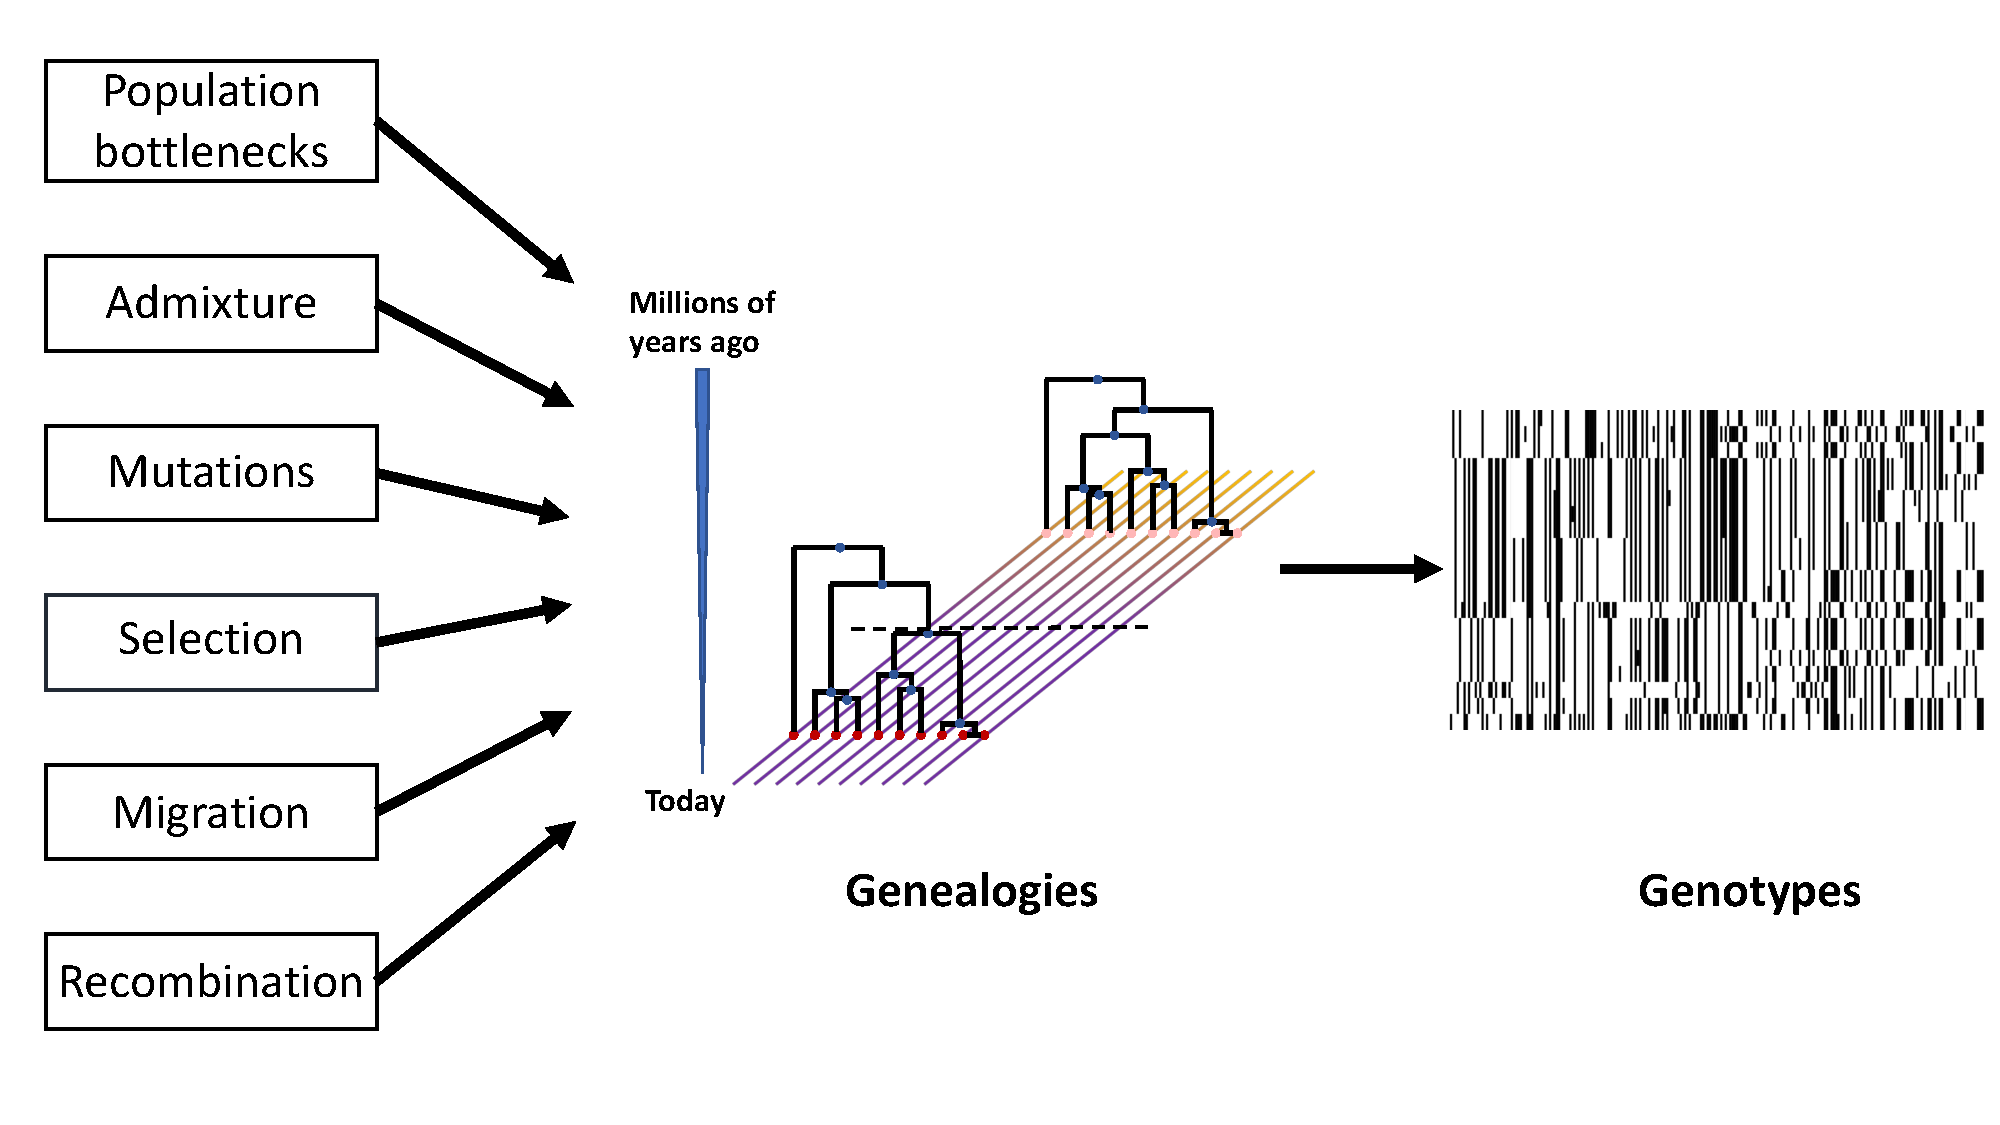
\includegraphics[width=\linewidth]{figures/thesis_ghostbuster_intro.pdf}
    \caption{\textbf{Evolutionary forces impact genotypes through genealogies.} Evolutionary forces like mutations, recombination, population bottlenecks, admixture, migration and selection affect the observed genotypes through the unobserved genealogies}
    \label{fig:ghostbuster_intro}
\end{figure}

Inferring Ancestral Recombination Graphs (ARGs) directly from genetic variation data is challenging because each recombination event splits the genealogical tree into two trees. The fact that mutation rates and recombination rates in humans (and many other species) are roughly similar means that, on average, there is only one mutation per branch on the tree, making it difficult to infer the genealogy. However, ARG inference methods leverage the fact that recombinations are unevenly distributed along the genome and still result in correlated adjacent trees. Over the past decade, new statistical methods have been developed to utilize these insights for ARG inference. 

ARG-weaver \cite{rasmussen2014genome} is one of the earliest scalable genealogy inference methods. ARG-weaver uses a Markovian approximation to the coalescent with recombination, the Sequentially Markovian Coalescent (SMC) \cite{mcvean2005approximating}, to constrain the space of possible ARGs. The SMC model reduces the search space of possible ARGs and makes it Markovian by ignoring coalescent events between lineages that do not share overlapping ancestral material. It essentially moves along the chromosome and updates the coalescent tree instead of the full ancestral recombination graph whenever a recombination occurs. ARG-weaver simplifies the inference of Ancestral Recombination Graphs (ARGs) by discretizing time, which further reduces the space of possible ARGs. It employs a Gibbs sampling approach, where a sample is threaded into the ARG based on the conditional probability of the rest of the ARG. Despite these approximations, ARG-weaver is limited in its scalability and can handle at most a few hundred samples.
% https://www.nature.com/articles/hdy201338
% McVean and Cardin (2005) 
% https://web.archive.org/web/20220517024716id_/https://www.biorxiv.org/content/biorxiv/early/2021/11/27/2021.11.15.468686.full.pdf

Tsinfer \cite{Kelleher2019} and tsdate \cite{wohns2022unified} are heuristic algorithms for ARG inference that are able to scale to hundreds of thousands of samples. Tsinfer uses a variation of the Li and Stephens algorithm to infer the tree sequence. It first estimates various possibilities of ancestral haplotypes at a given site and then uses the Li and Stephens copying process to paint the younger ancestors using older ancestors, thereby generating an ARG structure around the variant. Tsdate uses the topologies inferred using tsinfer to date the coalescence events using a conditional coalescent prior, conditioning on the number of descendants of each node on a local tree. Tsinfer and tsdate also demonstrated that storing genotype information in the tree sequence format saves a significant amount of disk space, leveraging the tree structure to save the variants instead of treating all variants independently.

Relate \cite{Speidel2019} is another heuristic algorithm for genealogy inference that scales to thousands of samples. Like tsinfer, Relate uses a variation of the Li and Stephens algorithm to infer the genealogies. It proceeds by using the Li and Stephens algorithm to calculate pairwise distances between samples at a given site, followed by hierarchical clustering to build a tree that best represents the observed variation around this site. Once the local trees are inferred and heuristically matched with adjacent trees, Relate estimates the coalescence times using an MCMC routine under the coalescent prior, conditioning on the tree topology. Relate also supports an iterative method to jointly estimate the population sizes along with estimating the coalescence times, making it more flexible for use in human datasets.

ARG-Needle \cite{zhang2023biobank} is a recent heuristic algorithm that is able to scale to hundreds of thousands of samples. Like ARGweaver, it threads a sample into the genealogy one at a time, but uses heuristics to speed up the process. It essentially proceeds as follows: for a new sample to be threaded, it detects \(K\) closely related samples around the variant, uses ASMC \cite{palamara2018high} to infer the coalescence times with those \(K\) possible samples, and then uses the sample corresponding to the minimum coalescence time to thread the new sample into the ARG. This process is repeated until all samples are threaded into the genealogy. Apart from genealogy inference, ARG-Needle also demonstrated the promise of using genealogies for phenotype prediction and association testing.

Singer \cite{deng2024robust} is a Bayesian method for ARG inference that scales to hundreds of samples. Like ARGweaver and ARG-Needle, Singer uses threading to infer the genealogies in a Bayesian way. Specifically, Singer employs a two-step threading algorithm where the first step samples the possible branch to thread and the second step samples the coalescence time for this threading. This is done under an MCMC routine, which enables the sampling of not only coalescence times but also tree topologies.

Overall, there has been recent development in accurate and scalable inference of genome-wide genealogies from genetic variation data. A comprehensive review comparing the performance of some of these ARG inference methods can be found in \cite{brandt2022evaluation}. This opens a new suite of directions to understand the evolutionary forces responsible for our genetic variation using these genealogies. In the next chapter, we survey some novel methods that rely on genealogies and help us understand our human past more accurately.

\subsection{Genome-wide genealogies to understand evolutionary history}

By inferring genome-wide genealogies, we hope to be one step closer to understanding evolutionary history, as the evolutionary history has impacted genetic variation through these genealogies. Let's explore the various evolutionary forces we can infer once we know the genealogies.

\textbf{Inferring population sizes using genealogies:} Under the coalescent, the population sizes are defined as the reciprocal of the coalescent rates between individuals in the same population. Therefore, given the genealogy, it is straightforward to infer the population sizes. A common approach to infer these time-varying population sizes is to discretize the time into several epochs and count the number of coalescence events between individuals in each epoch, divided by the opportunity for the coalescence event to happen, i.e., the sum of branch lengths in the epoch. In a simplistic case, this can be done for all pairs of individuals in the population, which results in an unbiased estimate of the population size.

\textbf{Inferring population structure using genealogies:} Following the argument for inferring population sizes, one can also infer cross-population coalescence rates, i.e., the chance of coalescence between two individuals from different populations. These rates are a common way to identify population structure or migration, as populations with higher cross-coalescence rates would be more similar to each other either due to a recent population split or recent migration between the two populations.

\textbf{Inferring presence of admixture using genealogies:} A simple way to identify recent admixture in a genealogy is by looking at genealogical nearest neighbors. If there is a recent admixture event, different regions of the genome would have different affinities to reference populations. A straightforward method to infer regions of the genome where a target individual is closer to one population than another is to look at its first coalescence event with the reference panel. A population description of the sister individuals at the tree would roughly indicate which population the target individual most closely relates to in that chapter of the genome. This is also how admixture inference methods like ChromoPainter work. A more careful analysis is needed if there are multiple admixture events or if the admixture event is old and can't be summarized by just the first coalescence event. Our method, GhostBuster (discussed in Chapters 2-4), addresses exactly this problem.

\textbf{Inferring positive selection:} Relate \cite{speidel2024high} devised a simple statistic to detect the presence of positive selection in the data. Specifically, the statistic compares the speed of spread of a certain lineage relative to other lineages in the tree. Relate's selection test uses results from the standard coalescent to model the joint distribution of the number of descendants given \(k\) lineages. Relate's selection test produced controlled false positive rates while outperforming other selection inference methods, such as singleton density scores \cite{field2016detection}, which did not leverage the genealogy to infer selection.

Among other applications, twigstats \cite{speidel2024high}, used inferred genealogies to more accurately estimate f-statistics. By effectively truncating trees and focusing only on mutations in the recent part of the tree, twigstats improved f-statistics standard errors to detect fine-scale structure. Another approach, introduced glike \cite{fan2023likelihood}, involves estimating the likelihood of the observed genealogy given the demographic parameters, thereby accurately estimating parameters like population sizes, admixtures, and migrations from the observed genealogies. This method surpasses techniques that only use genetic data for inference. A comprehensive review comparing different ARG inference methods and discussing their application in understanding human history can be found in \cite{brandt2024promise}.
% good review - https://academic.oup.com/gbe/article/16/2/evae005/7577593

\subsection{Motivation for GhostBuster}

% Paragraph 1 is Problem formulation (often combined with next paragraph)
% Paragraph 2 is Previous work on the problem (often combined with next paragraph)
% Paragraph 3 is Challenges that have yet to be solved
% Paragraph 4 is New approach to these challenges
% Paragraph 5 (optional) is Overview of results/interpretation (often
% combined with previous paragraph)

% Population demographic factors, such as population structure and migrations, have shaped the genetics of present-day samples, consequently affecting phenotypes. The advent of large-scale genomic datasets and theoretically grounded methods to analyze this data have enabled better understanding of this human population history. Previous methods for understanding human population history typically rely on deriving some summary statistics from genetic data to infer the presence of admixture and population structure. However, identifying subtle changes in population history directly from the genetic data is challenging, especially when there is minimal external evidence or when source groups remain unsampled. These are called ghost events or ghost populations. Large-scale inference of genome-wide genealogies has enabled a more direct examination of the demographic factors influencing genetics, resulting in more powerful inferences.

% In this thesis we propose a method, called GhostBuster, which utilizes genealogies to understand past demographic factors like migrations and admixtures more accurately and in a more interpretable manner. Through simulations and real-data examples, we demonstrate that GhostBuster can successfully recover signatures of both ancient and recent admixtures, accurately identifying source groups, admixture times, and local ancestry of target individuals. Notably, we infer a back-to-Africa migration that contributed up to 8\% Eurasian ancestry to sub-Saharan Africans between 5,000 and 15,000 years ago. Additionally, we identify and characterize a deep admixture event in Africa involving ghost populations, which split around 300,000 years ago and mixed within the last 50,000 years to form the present-day sub-Saharan African populations.

% Demographic factors - population structure, migration, admixture
% Cite previous methods
% Examples of events which are not well characterized
% Methods like globetrotter can resolve recent history 1000-2000 years ago
% ancient DNA has extended it to several 1000 years
% archaics 50k years, but adna is limited and difficult to get older in time
% making inferences about deep human past difficult


% Mention GB is a mixture model, clusters trees


Population movements and mixtures have been a constant feature of human history across various time scales. Notable examples include the Out of Africa migration, Neanderthal and Denisovan introgression over 40,000 years ago, multiple admixtures in Holocene Europe, and recent migrations and multi-way admixtures in the Americas within the last few hundred years (see Figure \ref{fig:gb-intro}a-c). Despite this, the genetic legacy of some events, particularly older ones, remains elusive due to the limited resolution of statistical methods and the scarcity of ancient DNA samples (see Figure \ref{fig:gb-intro}d).

Many previous methods for deciphering admixtures have relied on detecting long segments of DNA corresponding to recent admixture events. These methods often use linkage disequilibrium (LD) decay curves to date admixtures, which have proven effective for identifying events within the last few thousand years. However, as recombination events shorten these segments, the statistical power of these methods diminishes, making it challenging to infer older admixtures \cite{hellenthal2014genetic, loh2013inferring, moorjani2011history, patterson2012ancient}. Another widely used approach involves sequencing ancient DNA samples, providing direct evidence of the genetic makeup of our ancestors. Ancient DNA studies, employing methods such as PCA \cite{Patterson2006}, STRUCTURE \cite{Pritchard2000}, and f-statistics \cite{reich2009reconstructing,reich2012reconstructing,patterson2012ancient,haak2015massive,durand2011testing}, have significantly extended our understanding of human history up to approximately 10,000 years ago—beyond the temporal reach of LD-based methods. However, the deeper human past remains difficult to uncover due to the scarcity of ancient DNA samples from earlier periods, which are challenging to preserve over such long timescales. While the limited number of archaic DNA samples has offered some insights, they remain insufficient to fully reconstruct the complex genetic history of early human populations.

Furthermore, previous methods typically rely on deriving summary statistics from genetic data to infer the presence of admixture and population structure. Identifying subtle changes in population history directly from genetic data is particularly challenging when there is minimal external evidence or when source groups remain unsampled. The large-scale inference of genome-wide genealogies provides a more direct approach to examining the demographic factors influencing genetic variation. By modeling these demographic changes, genealogies offer a more interpretable and detailed view of human history, allowing researchers to trace population dynamics with greater accuracy and uncover previously hidden aspects of our ancestral past.

In this thesis, we introduce a novel method called GhostBuster, which leverages coalescent theory and inferred genealogies to analyze past mixture events with enhanced precision and interpretability. GhostBuster is a mixture model that clusters local trees within genealogies based on coalescence rates between a target lineage and a set of reference populations. This approach not only characterizes mixture events but also decomposes the local ancestry of target individuals. Unlike traditional methods, GhostBuster does not require sampled source populations to identify admixture events, making it capable of detecting ghost admixtures. Through simulations and real-data examples, we demonstrate that GhostBuster can successfully recover signatures of both ancient and recent admixtures, accurately identifying source groups, admixture times, and the local ancestry of target individuals.

We applied GhostBuster to both modern and ancient samples from sub-Saharan Africa, a region where ancient DNA is particularly scarce due to environmental conditions that hinder DNA preservation. Our analysis uncovered two significant events that occurred more than 5,000 years ago in Africa. First, we identified a back-to-Africa migration event that introduced up to 8\% Eurasian ancestry into all sub-Saharan African populations we analyzed. This event, occurring between 5,000 and 15,000 years ago, helps explain the presence of small amounts of Neanderthal ancestry in modern Africans. We further validated this admixture by examining specific mutational profiles and characterized the event by identifying the source population and detecting signatures of positive selection. Second, we uncovered a deep admixture event corresponding to the pre-Out of Africa population structure. Our findings indicate the existence of two major populations in Africa over 100,000 years ago, one of which contributed significantly to the population that eventually migrated out of Africa. Present-day Africans are admixtures of these two ancient populations, which split around 300,000 years ago. We also found differences in the affinities of these ancient populations with other archaic humans from that period. Lastly, we observed that the two ancient populations exhibit different levels of polygenic score (PGS) portability, correlating with their genetic affinity to the Out of Africa population.


% advantage of looking at genealogy







\begin{figure}[h!]
    \centering
    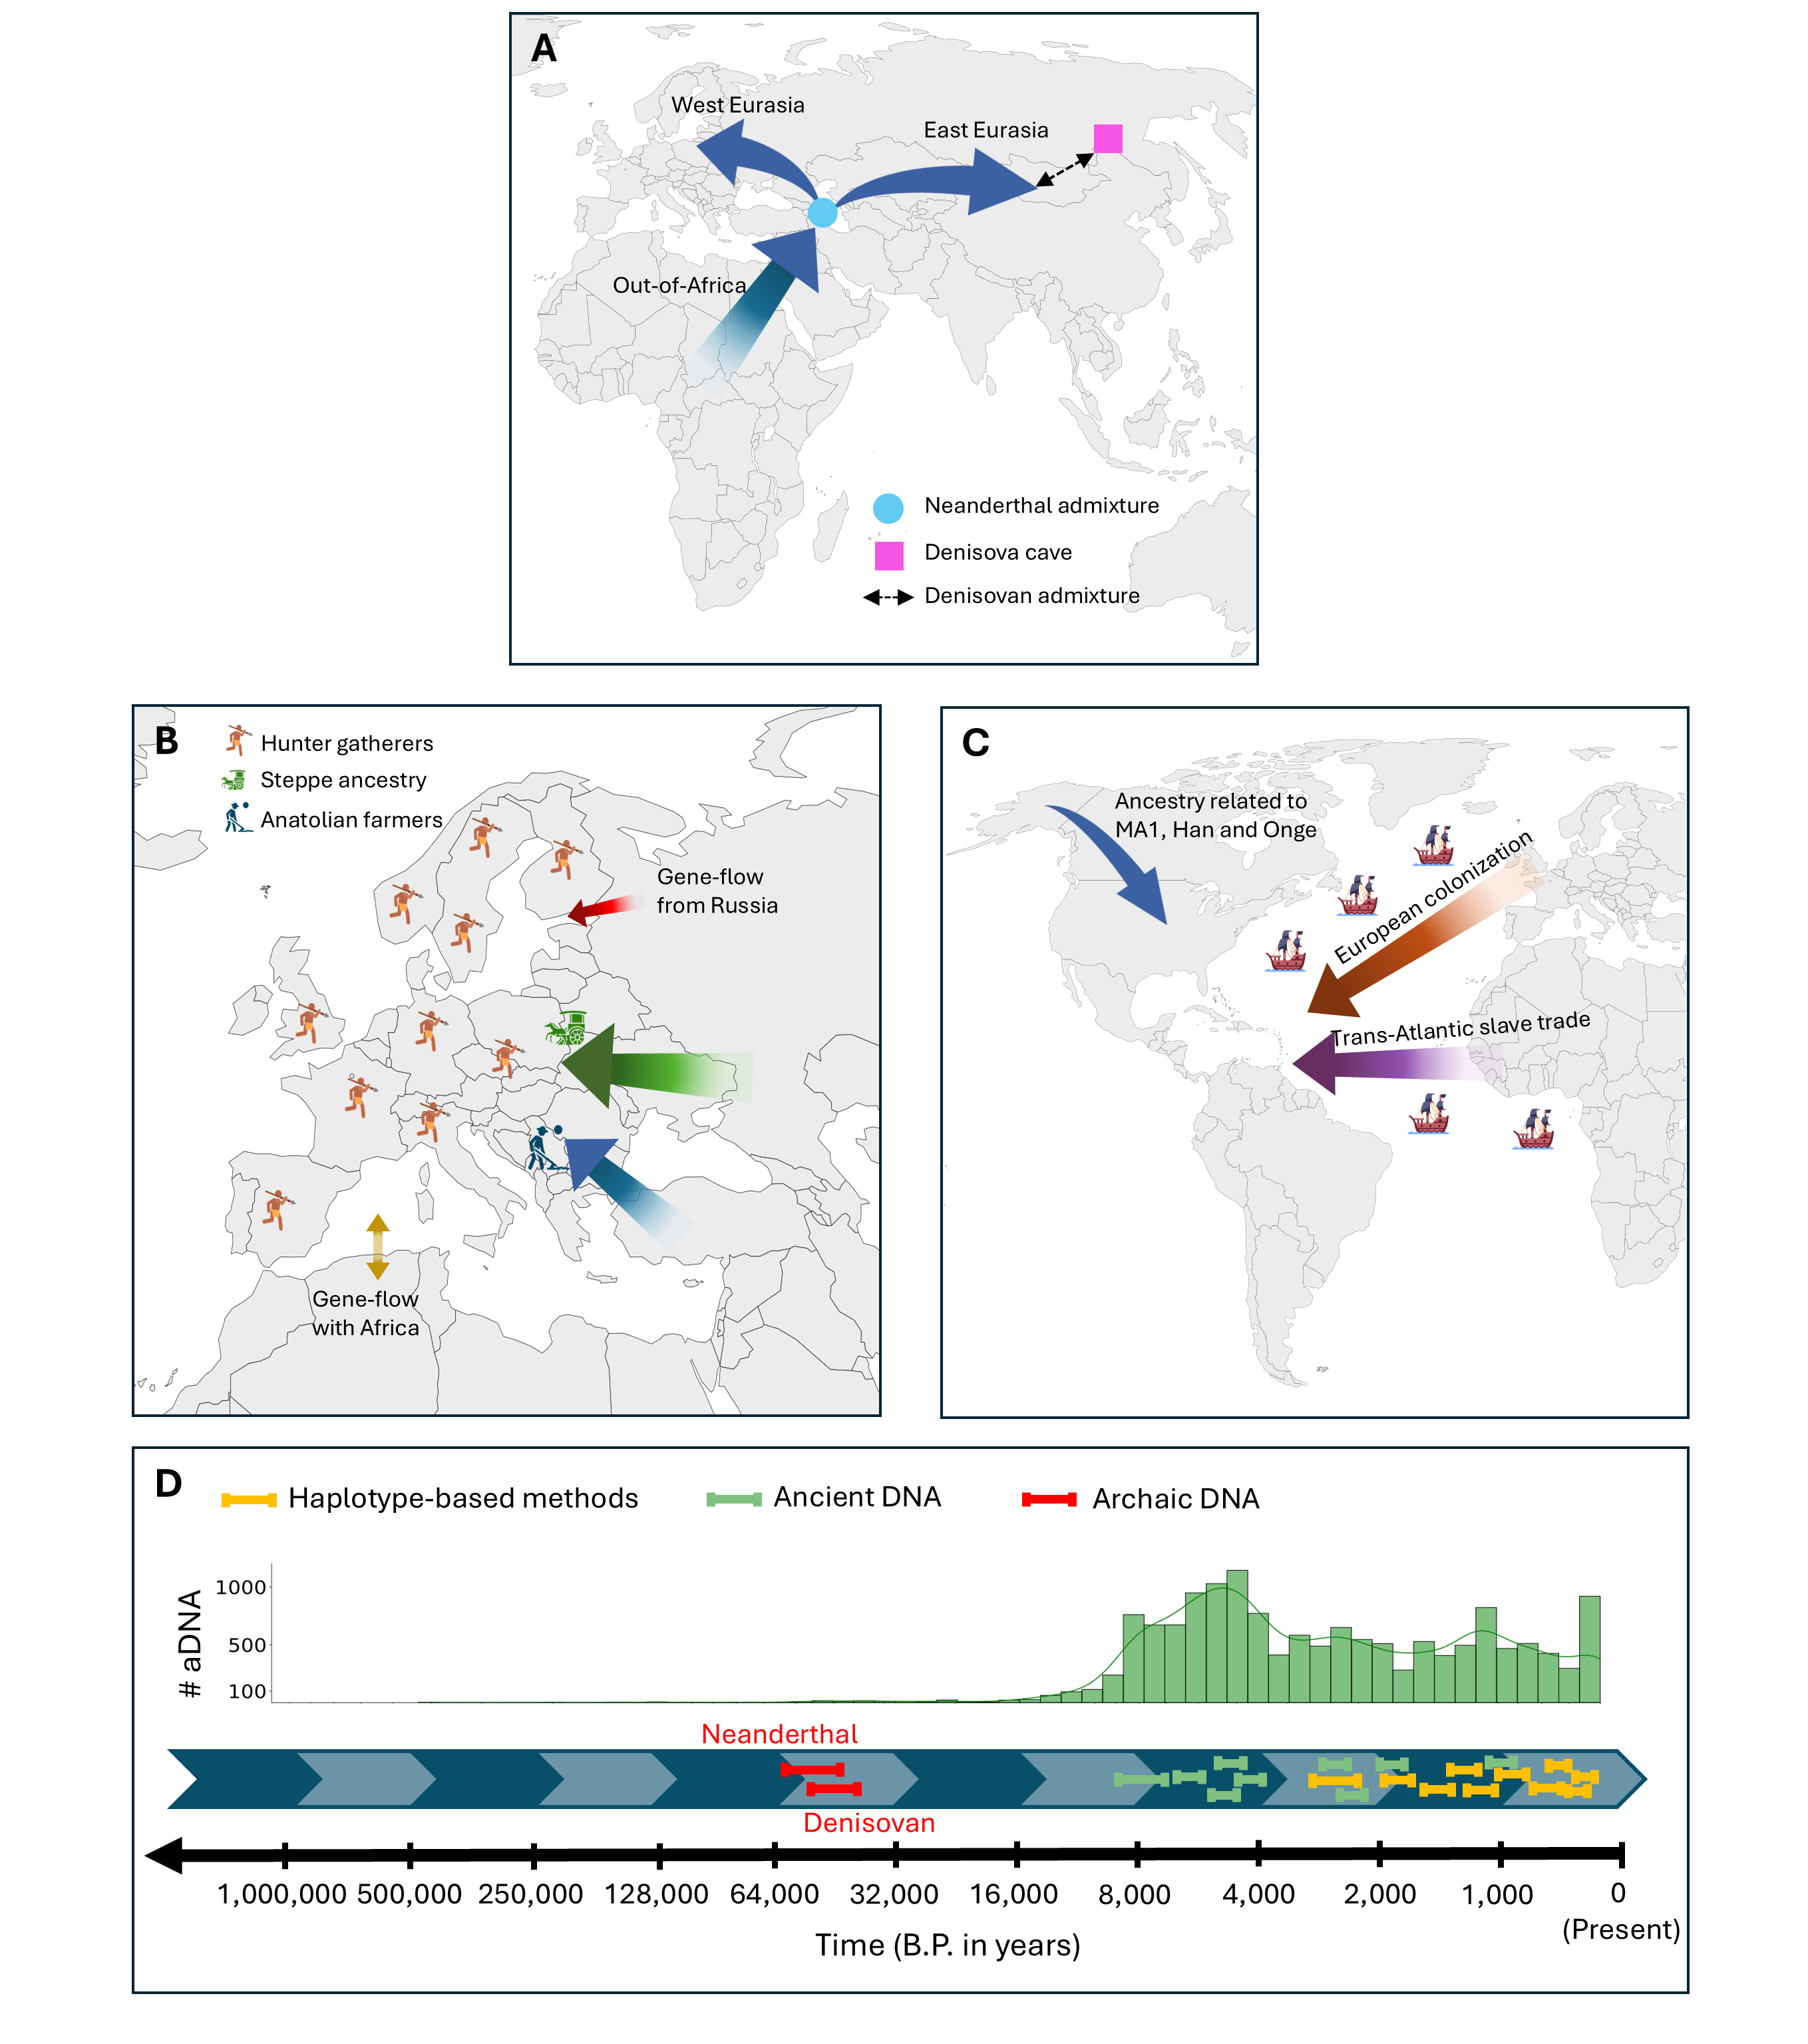
\includegraphics[width=\textwidth]{figures/thesis_gb_migration_example_v2.png}
    \captionsetup{width=\textwidth+3cm}
    \caption{
    \footnotesize
    \textbf{Some examples of migration and admixture events in human history.} A. Archaeological and genetic evidence suggests modern humans originated in Africa and migrated out between 50,000 and 100,000 years ago \cite{darwin1874descent, lopez2015human}. They interbred with Neanderthals, contributing up to 3\% of non-African DNA. After leaving Africa, the population split into west and east Eurasian groups, creating genetic differences between Europeans and Asians. East Eurasians also admixed with Denisovans, though the timing and location are debated \cite{jacobs2019multiple, reich2010genetic}.
    %
    B. Europe has experienced significant migrations, starting with Anatolian farmers 7,000-9,000 years ago, followed by Steppe pastoralists around 5,000 years ago, which heavily influenced present-day European ancestry. There is also evidence of recent gene flow from North African groups into southern Europeans, such as Italians and Spanish, and ancient Siberian-related ancestry in northeastern Europeans like Finns and Russians \cite{haak2015massive, salter2019fine}.
    %
    C. The peopling of America likely began during the last glacial period, which created a land bridge to Eurasia \cite{severinghaus1999abrupt}, ending around 15,000 years ago. Ancient DNA in America shows genetic links to ancient Siberians (MA1), Han Chinese, and the Onge tribe \cite{skoglund2016genomic}. Present-day American genetics are influenced by historical events like colonization and the trans-Atlantic slave trade, resulting in admixture from Native American, African, and European sources \cite{smith2004high, price2009sensitive}.
    %
    D. Previously identified human admixtures were determined using various methods, including haplotype-based approaches \cite{hellenthal2014genetic, loh2013inferring, moorjani2011history, patterson2012ancient}, ancient DNA, and archaic DNA analyses. The histogram shows the ages of ancient DNA samples sequenced to date, sourced from the Allen Ancient DNA Resource \cite{mallick2024allen}.
    }
    \label{fig:gb-intro}
\end{figure}

%% add timeline to the figure

\clearpage

\section{Understanding complex traits through genetic data}

An important line of work in statistical genetics focuses on understanding how the patterns of genetic variation in present-day individuals affect phenotypes. The first disease gene was mapped in 1983, identifying a polymorphism on chromosome 4 responsible for Huntington's disease \cite{Gusella1983}. This study involved analyzing pedigrees with fewer than 100 samples to pinpoint the genetic cause of Huntington's disease. Huntington's disease is an example of a monogenic disorder, where a single alteration in the genome explains the entire genetic basis of the disease. With the growing size of genetic datasets, we now know that most traits and diseases in humans are not monogenic but polygenic, where hundreds or thousands of small alterations in the genome explain the genetic basis of a trait. Finding these small polygenic effects spread across the genome requires examining genetic variation data genome-wide in a larger number of samples.

The Wellcome Trust Case Control Consortium (WTCCC) \cite{WTCCC2007} was one of the first efforts to perform a large-scale genetic association study. It genotyped 17,000 individuals, comprising 2,000 cases and 3,000 common controls across seven common diseases (type 1 diabetes, type 2 diabetes, coronary heart disease, hypertension, bipolar disorder, rheumatoid arthritis, and Crohn's disease). The WTCCC performed a genome-wide association study to look at polymorphisms in the genome that correlate more than usual with the case-control status and found 90 new variants across all the diseases analyzed, confirming the presence of 28 previously established variants. Since then, Genome-wide association studies have become a cornerstone in current-day quantitative genetics to understand how genetic variation affects phenotypes.


\subsection{Basic definitions}

Heritability of a trait, roughly speaking, is the proportion of total variance explained by genetic variants. It measures how important genetics are in predicting a given trait, where a heritability of 1 means genetics explain all the variance in the trait between individuals, and a heritability of 0 means genetics do not explain any variance in the trait. It is important to note that heritability for a trait depends on the quality of phenotypic measurements and the environment itself. Heritability should not be confused with the variance associated with the direct biological mechanisms affecting a trait. In many complex traits, the path from genes to traits is complex and indiscernible \cite{Neale2017}. A more detailed understanding of heritability, its implications, and common misunderstandings can be found in \cite{Visscher2008,Gusev2021}.
% http://www.nealelab.is/blog/2017/9/13/heritability-101-what-is-heritability#:~:text=For%20example%2C%20the%20heritability%20of,all%20the%20relevant%20genetic%20effects).
% http://gusevlab.org/projects/hsq/

Linkage disequilibrium (LD) refers to the correlation patterns in genetic variation data due to the fact that variants close to each other are transmitted together more frequently than variants further away from each other. LD is further exacerbated because most recombination in humans happens at recombination hotspots, creating distinct LD patterns along the genome. LD can be both a boon and a bane in analyzing human variation data. It is a boon because common variants can capture the signal from nearby rare variants, which are usually causal for a given trait, thus improving the power of predicting the phenotype using the variation data. However, it is a bane because the same LD makes it challenging to distinguish causal variants from associated variants, as tightly correlated variants obscure the identification of the true causal variant.

Two of the major challenges in performing genome-wide association studies are the presence of population structure and relatedness in the data, which confound the genetic signals, inflating the test statistics. We have already discussed population structure in chapter 1.2.1. Relatedness, often referred to as kinship, is estimated through the genetic relatedness matrix (GRM) and is computed as \(\frac{XX^T}{M}\), where \(X\) is an \(N \times M\) genotype matrix, \(N\) is the sample size, and \(M\) is the number of variants. The GRM forms an essential part of linear mixed model methods to perform genome-wide association studies, which will be discussed further in chapter 1.3.3.


\subsection{Genome-wide association studies: usage and applications}

After it became clear that many human traits are polygenic in nature, an unbiased genome-wide scan for variants associated with these traits was warranted. Following the first large-scale genome-wide association study published by the Wellcome Trust Case Control Consortium (WTCCC) in 2007, a huge wave of large-scale population-wide studies aimed at understanding the genetic architectures of various complex traits ensued. Today, 17 years after WTCCC, GWAS has become a standard protocol for understanding the genetic basis of most complex traits. With sequencing and phenotyping efforts from pharmaceutical industries, academia, and independent nation-wide `biobanks', GWASs have been performed on thousands of human traits, using millions of individuals, and have identified hundreds of thousands of genetic associations \cite{GWASCatalog}. %GWAS catalog

GWAS has become a vital element in drug discovery, with two-thirds of the new drugs approved by the FDA in 2021 supported by human genetic evidence \cite{rusina2023genetic,ochoa2022human,abdellaoui202315}. Some examples include Finerenone, an NR3C2 antagonist approved for the treatment of chronic kidney disease \cite{teumer2019genome,bakris2020effect}. Baricitinib, identified through GWAS studies for COVID-19 severity, was shown to reduce the COVID-19 mortality rate by approximately 20\% \cite{favalli2020baricitinib,horowitz2022genome}. It is important to note that GWASs are not enough to support drug target discovery on their own. Further downstream analysis, such as replication, expression QTL studies in relevant tissues and cell types, and understanding off-target effects, are necessary and are part of the GWAS pipeline to obtain suitable drug targets before a randomized control trial.
% https://www.nature.com/articles/s41467-019-11576-0

Apart from identifying genetic associations with traits, GWAS is also utilized to build polygenic scores for a trait or disease susceptibility. Polygenic scores, or PGS, use the estimated effects for a trait to build a predictor of the genetic likelihood of a trait. PGS have found clinical potential for personalized medicine and treatment, with current utility for various genetic disorders including cardiovascular diseases \cite{torkamani2018personal}. GWAS has also enabled the identification of genetic similarity between traits and diseases, helping to identify biological pathways for gene functions \cite{solovieff2013pleiotropy}. On a more general level, GWAS hits have also helped us understand the evolution of certain human traits, where selection mechanisms like directional, stabilizing, and pleiotropic are among the most likely explanations of how trait-associated variants spread forward in time. Additionally, GWAS has been useful in causal inference studies, as a genetic instrument in Mendelian randomization, helping to identify disease-causing traits. An overview of the GWAS pipeline and its application can be found in Figure \ref{fig:qd-intro} and following reviews \cite{visscher201710, abdellaoui202315}.

\begin{figure}[h!]
    \centering
    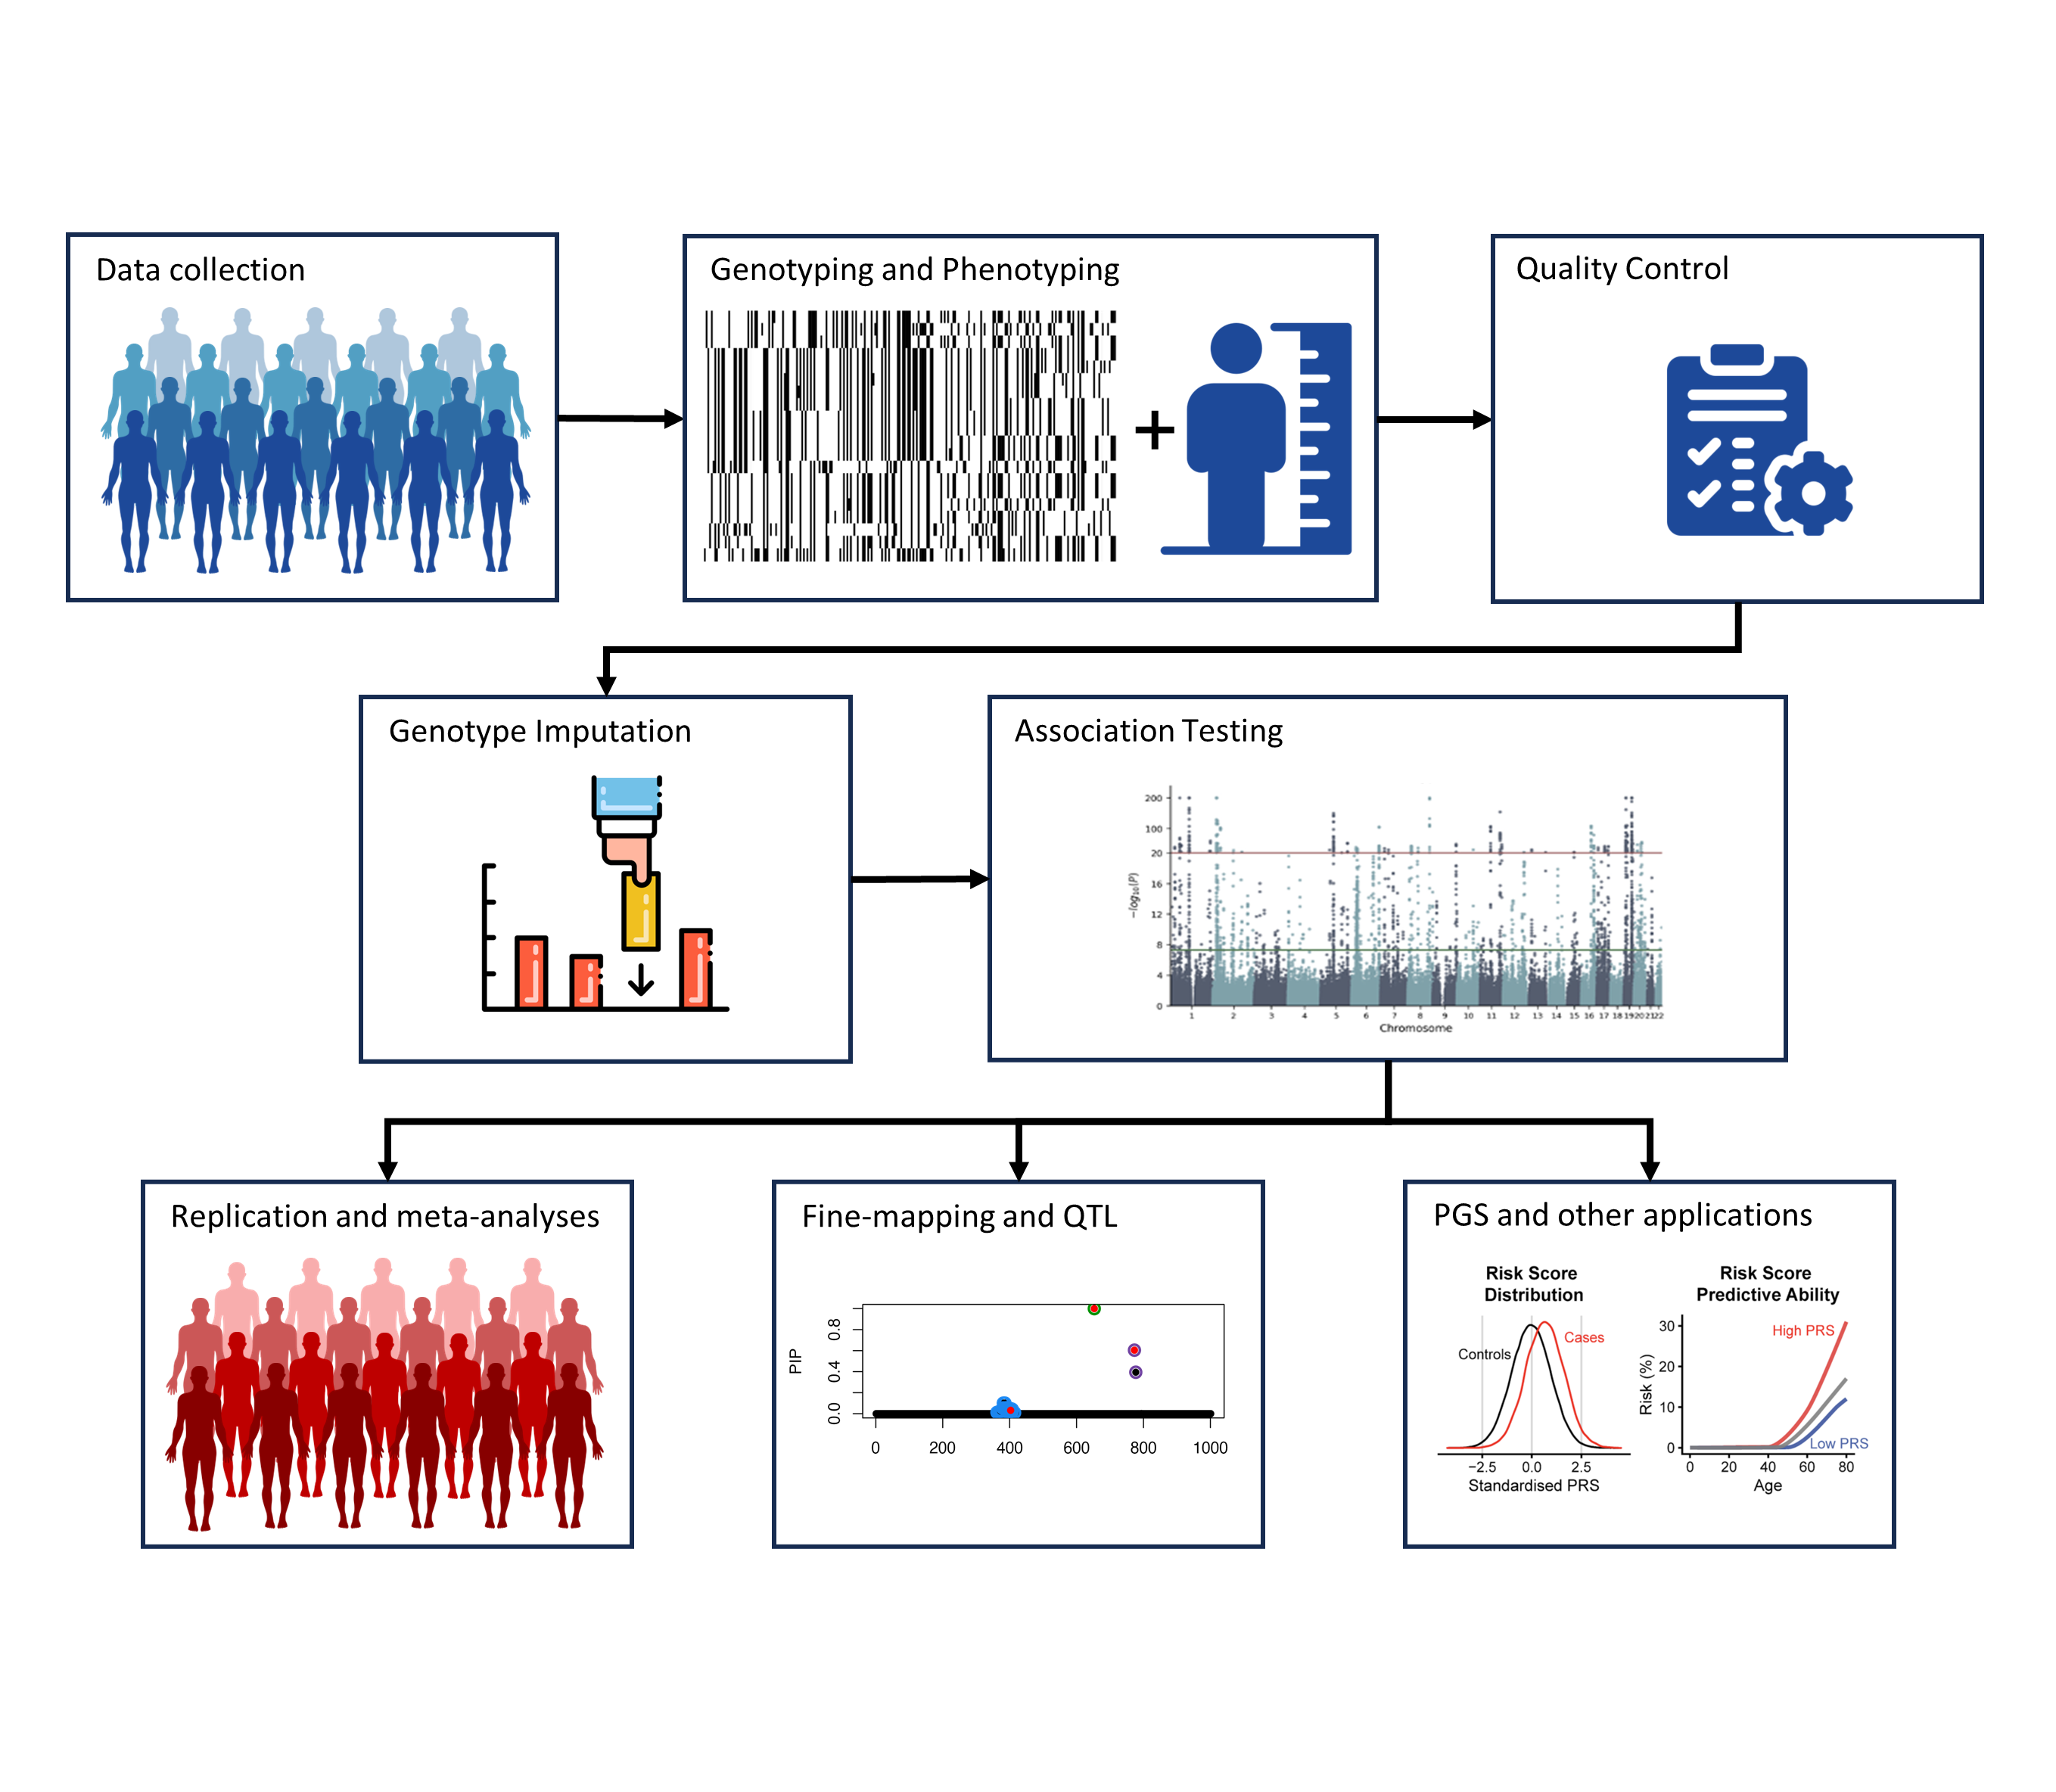
\includegraphics[width=\textwidth]{figures/thesis_qd_gwas_pipeline.png}
    \caption{
    \textbf{Overview of a typical GWAS pipeline.} The GWAS pipeline typically begins with genotyping and phenotyping a large cohort of individuals, including both cases and controls for disease traits. Genotyping can be conducted using either low-cost SNP arrays or whole-genome sequencing. Quality control steps are crucial and involve filtering variants and samples based on various criteria (see section \ref{sec:ch5-data} for detailed quality control procedures). If genotyping was performed instead of whole-genome sequencing, genotype imputation follows as the next step. Subsequently, genome-wide association testing is conducted for each variant and phenotype of interest to generate p-values and effect estimates, indicating the association between each variant and the phenotype. The resulting GWAS summary statistics have several downstream applications. These include replication and meta-analyses to enhance statistical power, fine-mapping and functional analyses to identify causal variants among the associated variants, and the calculation of polygenic scores. This pipeline structure was adapted from \cite{uffelmann2021genome}, with the fine-mapping figure from \cite{Wang} and the polygenic scores figure from \cite{wand2021improving}.
    }
    \label{fig:qd-intro}
\end{figure}

\subsection{Theoretical framework to perform GWAS}
\label{sec:ch1-lmm}
There are two main categories of methods to perform genome-wide association studies. The first set of methods involves fitting a linear model to estimate the effect of a variant on the phenotype, taking into account various covariates. The linear models fit the following model:
\begin{equation}
    y = x_{test}\beta_{test} + \alpha C + \epsilon. \label{linear}
\end{equation}
In the above, \(y\) is an \(N \times 1\) vector of mean-centered and standardized phenotype values, \(x_{test}\) is an \(N \times 1\) vector of mean-centered and standardized biallelic variant values (i.e., the original \(\tilde{x}_{test}\) takes values in \(\{0,1,2\}^N\) for diploid samples), \(C\) is an \(N \times C\) matrix of covariates of interest, such as principal components, age, and sex, and \(\epsilon\) is Gaussian noise.

Linear models fit the model in equation \ref{linear} using a simple OLS estimate for linear regression or an iterative scheme for logistic regression. Test statistics are calculated from standard closed-form solutions for the standard error of the estimates. Although simple, linear models fail to correct for the presence of population structure and cryptic relatedness in the data, making the resulting test statistic estimates inflated. Therefore, methods that rely on linear models subset to only using unrelated and homogeneous subsets of data to ensure the false positive rates aren't too high. This, in turn, reduces the sample size and power to detect genetic associations in the dataset.

The second class of methods are Linear mixed models or LMMs. LMMs are an extension of linear models that facilitate the analysis of non-independent data. They are commonly adopted in the analysis of genomic data involving population structure or cryptic relatedness. LMMs handle non-independence by modeling random effects that capture variability within different subpopulations or phenotypic correlation across close relatives. In an LMM for genome-wide association analysis, the phenotype of interest is often modeled as a combination of fixed effects, which include the effects of the test variant and covariates, and random effects, which include genetic effects and environmental effects:
\begin{equation}
    y = x_{test}\beta_{test} + \alpha C + g + \epsilon \label{lmm}.
\end{equation}
Similar to the linear model above, $y$ is an $N \times 1$ vector of mean-centered and standardized phenotype values, $x_{test}$ is an $N \times 1$ vector of mean-centered and standardized biallelic variant values, $C$ is an $N \times C$ matrix of covariates.
%
We are mainly interested in inferring the fixed effect of a particular variant, $\beta_{test}$, given the random genetic effects, which help capture the effects of population structure and relatedness.
%
We model the genetic and environmental effects using
\begin{align}
    g &= \beta_{GRM} X_{GRM} \nonumber \\
    \epsilon &\sim  \mathcal{N}(0, \sigma^2_e) \label{lmm-1},
\end{align}
where $X_{GRM}$ is an $N \times M_{GRM}$ standardized genotype matrix and $\sigma^2_e$ is the environmental variance for a given phenotype.
%
For simplicity, the environmental random effect is assumed to be independent and identically distributed (i.i.d.) from a normal distribution, and the random genetic effect is modeled as a weighted sum of standardized genotypes. The random genetic effect $g$ can also be thought of as a sample from $\mathcal{N}(0, \sigma^2_g K)$, where $\sigma^2_g$ is the genetic variance for a given phenotype and $K = \frac{1}{M}X_{GRM}X_{GRM}^T$ is the genetic relatedness matrix.




\textbf{Leave-one-chromosome-out: }
%
It has been observed that in order to avoid reducing the power of association, the matrix $X_{GRM}$ should not contain the test variant $x_{test}$, as well as any other variants in linkage disequilibrium (LD) with $x_{test}$.
%
This problem has been referred to as ``proximal contamination'' \cite{listgarten2012improved}.
%
Fitting an LMM with genetic effects from variants not in LD with the testing variant, however, would require re-training the model to infer genetic effects for every tested variant, which would cause major computational overheads.
%
\cite{yang2014advantages} proposed a simple solution to this problem, referred to as the leave-one-chromosome-out (LOCO) scheme, where the $X_{GRM}$ is constructed using all variants except those on the same chromosome as the test variant.
%
For example, assuming $22$ autosomal chromosomes and a test variant on chromosome $7$, $X_{GRM}$ is built to contain all variants from chromosome $1$-$6$ and $6$-$22$.
%
This approach, which requires training a separate model for each chromosome, allows circumventing proximal contamination while increasing association power, and has been widely adopted by recent LMM association algorithms \cite{loh2015efficient,loh2018mixed,jiang2019resource}.
%
% Previous methods train 22 models (one per leave-one-chromosome) in parallel to estimate the effect estimates $\beta_{GRM}$ for each LOCO model and use them to calculate the test-statistics by choosing the correct LOCO model. 

\textbf{Calculation of the test statistic: }
%
To infer the fixed effect $\beta_{test}$ in Equation \ref{lmm}, one can marginalize the random effects $\beta_{GRM}X_{GRM}$ and $\epsilon$ to get the marginalized log-likelihood:

\begin{align}
    y \mid x_{test}, \beta_{test}, \sigma_e^2, \sigma_g^2 &\sim \mathcal{N}(x_{test}\beta_{test}, \frac{\sigma_g^2}{M} X_{GRM}X_{GRM}^T + \sigma_e^2 I_N) \nonumber \\
    \log P(y \mid x_{test}, \beta_{test}, \sigma_e^2, \sigma_g^2) &\propto -\frac{1}{2} (y-x_{test}\beta_{test})^TV^{-1}(y-x_{test}\beta_{test}) -\frac{1}{2} \lvert \log(V) \rvert,
\label{eq:full_like}
\end{align}

where $\sigma_g^2$ and $\sigma_e^2$ are genetic and environmental variance components as described above, and $V$ is a covariance matrix, defined as $V = \frac{\sigma_g^2}{M} X_{GRM}X_{GRM}^T + \sigma_e^2 I_N$.
%
The maximum likelihood estimate (MLE) for $\beta_{test}$ is obtained by setting $\frac{\partial \log P(y \mid x_{test}, \beta_{test})}{\partial \beta_{test}} = 0$; the variance of the estimate is obtained using the inverse Fisher information $ -\mathbf{}{E}\left[\frac{\partial ^2 \log P(y \mid x_{test}, \beta_{test})}{\partial \beta_{test}^2} \mid \hat{\beta}_{test}\right]^{-1}$ and takes the form

\begin{align}
    \hat{\beta}_{test} &= (x_{test}^T V^{-1} x_{test})^{-1}(x_{test}^T V^{-1} y) \nonumber \\
    var(\hat{\beta}_{test}) &=(x_{test}^T V^{-1} x_{test})^{-1} \label{lmm-inf}.
\end{align}

%
The variance components, $\sigma_g^2$ and $\sigma_e^2$, are estimated using restricted likelihood maximization (REML) \cite{loh2015efficient} or moment-based methods \cite{wu2018scalable,pazokitoroudi2020efficient} rather than standard maximum likelihood estimation.
%
In this work, we estimate the variance components $\hat{\sigma}_g^2$ and $\hat{\sigma}_e^2$ using the RHE-MC algorithm \cite{wu2018scalable,pazokitoroudi2020efficient}, a highly scalable moment-based approach that was recently extended to allow processing multiple traits in parallel \cite{yiorgos2023,alma991025317822307026}.
%
We then estimate the covariance matrix using $\hat{V} = \frac{\hat{\sigma}_g^2}{M} X_{GRM}X_{GRM}^T + \hat{\sigma}_e^2 I_N$, and the effects using

\begin{align}
    \hat{\beta}_{test} &= (x_{test}^T \hat{V}^{-1} x_{test})^{-1}(x_{test}^T \hat{V}^{-1} y), \nonumber \\
    var(\hat{\beta}_{test}) &= (x_{test}^T \hat{V}^{-1} x_{test})^{-1} \label{lmm-inf2}.
\end{align}

%
Using the asymptotic property of the MLE, 

\begin{equation}
   \frac{\hat{\beta}_{test} - \beta_{test}}{\sqrt{var(\hat{\beta}_{test})}} \sim \mathcal{N}(0, 1) 
\end{equation}

%
To test the null hypothesis $\beta_{test} = 0$, we therefore substitute the MLE estimate and the variance of the estimate from Equation \ref{lmm-inf2}, and square both sides to get:

\begin{equation}
   \frac{(x_{test}^T \hat{V}^{-1} y)^2}{x_{test}^T \hat{V}^{-1} x_{test}} \sim \chi^2_1 \label{lmm-chi2}.
\end{equation}


There are two main modelling assumptions about the distribution of genetic effects along the genome, which distinguishes LMMs into two categories: Infinitesimal and non-infinitesimal models. 

%
\textbf{Infinitesimal model: }
%
The infinitesimal model places a normal prior on the effect estimates $\beta_{GRM}$ from Equation \ref{lmm-1}, and assumes the total genetic effect explained by all the genetic markers to be $\sigma_g^2$:
%

\begin{equation}
    \beta_{GRM} \sim \mathcal{N}(0, \sigma_g^2 I_M/M)
\end{equation}

%
As the prior and likelihood are conjugate, we can infer the posterior distribution $P(\beta_{GRM} \mid X_{GRM}, y)$:

\begin{equation}
    \begin{split}
        P(\beta_{GRM} \mid X_{GRM}, y) = \mathcal{N}\Bigg( &\left( \frac{I_M M}{\sigma_g^2} + \frac{X_{GRM}^T X_{GRM}}{\sigma_e^2} \right) ^{-1} \frac{X_{GRM}^T y}{\sigma_e^2}, \\
        &\left( \frac{I_M M}{\sigma_g^2} + \frac{X_{GRM}^T X_{GRM}}{\sigma_e^2} \right) ^{-1} \Bigg) \label{lmm-inf3}
    \end{split}
\end{equation}

%
The maximum-a-posteriori (MAP) estimate of $\beta_{GRM}$ in Equation \ref{lmm-inf3}, also referred to as the best linear unbiased predictor (BLUP), can be written as:

\begin{equation}
    \hat{\beta}_{GRM} = \left( \frac{I_M M}{\sigma_g^2} + \frac{X_{GRM}^T X_{GRM}}{\sigma_e^2} \right) ^{-1} \frac{X_{GRM}^T y}{\sigma_e^2} 
\end{equation}

%
The residual phenotype, formed by regressing out the effect of other variants on the phenotype, is given by $\tilde{y} = y - X_{GRM} \hat{\beta}_{GRM}$ and simplifies to

\begin{equation}
    \tilde{y} = y - X_{GRM} \hat{\beta}_{GRM} = \sigma_e^2 V^{-1} y
    \label{blup_lmm_link}
\end{equation}

%
This provides a link between the BLUP and test statistics for $x_{test}$ in Equation \ref{lmm-chi2}, which is exploited to compute test statistics for non-infinitesimal models.
%
Under the infinitesimal model, the test statistic can be rewritten as

\begin{equation}
    \frac{(x_{test}^T \tilde{y}/\sigma_e^2)^2}{x_{test}^T \hat{V}^{-1} x_{test}} \sim \chi^2_1
    \label{blup_lmm}
\end{equation}

%
% Write about the frequentist approach, prior on $\beta_{GRM}$ and chi-square test statistics derivation
% Derive the BLUP estimates and show how the numerator in chi-square is related to phenotype residual
%
\textbf{Non-infinitesimal model: }
%
It is often the case that a large fraction of variants are not linked to the phenotype, so the above model can be improved by adopting a more appropriate prior, such as a spike-and-slab prior, or a mixture-of-Gaussians prior.
%
The spike-and-slab prior can be modelled as follows:

\begin{equation}
P(\beta_{GRM}) \sim p_0 \mathcal{N} (0, \sigma_g^2/Mp_0) + (1-p_0) \delta(0),
\end{equation}

where $\delta(0)$ is the Dirac-delta function at $0$.
%
A mixture-of-Gaussians prior replaces the Dirac-delta function using a low-variance normally distributed component, and can be written as

\begin{equation}
P(\beta_{GRM}) \sim p_0 \mathcal{N} (0, \sigma_{g,1}^2/M) + (1-p_0) \mathcal{N} (0, \sigma_{g,2}^2/M).
\end{equation}

%

%
Equation \ref{blup_lmm} can still be used to compute test statistics, by replacing $\tilde{y}$ with the phenotype residuals calculated using BLUP under the non-infinitesimal model.
%
Note that it is often not possible to obtain a closed-form solution for the BLUP under an non-infinitesimal model, but can be approximated through MCMC or variational inference algorithms.

\subsection{Survey of methods to perform GWAS}

Plink \cite{purcell2007plink} is one of the most widely used linear model-based GWAS algorithms. Its subsequent versions \cite{chang2015second} improve its scalability by implementing vectorized operations over phenotypes, working with the disk-space efficient pgen format, and supporting sparse matrix multiplication \cite{rivas2024efficient}. Despite its efficiency, Plink does not implement a linear mixed model to correct for population structure and relatedness, and therefore is only used with unrelated homogeneous subsets of the data.

EMMA \cite{kang2008efficient} is among the earliest methods to implement a linear mixed model for association testing in human datasets. It optimized the fixed effects by maximizing the full likelihood in equation \ref{eq:full_like} relying on spectral decomposition. The overall algorithm was still cubic in sample size and required constructing the \(N \times N\) kinship matrix. EMMAX, or EMMA expedited \cite{kang2010variance}, was a follow-up to EMMA which improved its scalability by more than two orders of magnitude. Instead of recomputing the variance parameters for each variant separately, EMMAX observed that a single variant does not have a huge effect on the variance components and therefore estimated it once and reused it for association testing.

Fast-LMM \cite{lippert2011fast} used the spectral decomposition of the kinship matrix and its low-rank representation to speed up association testing further compared to EMMAX. Fast-LMM-Select \cite{listgarten2013fast} followed as a subsequent method, which subsets the markers for kinship calculation based on their predictability for the trait using a linear model. It was later shown that this strategy of reducing the number of markers in kinship calculation leads to inflation in the test statistics, as background polygenic effects aren't fully captured \cite{yang2014advantages}.

BOLT-LMM \cite{loh2015efficient,loh2018mixed} was one of the first methods to scale linearly with the number of markers and sub-quadratically with the number of samples. The overall complexity of BOLT-LMM was \(O(MN^{1.5})\). BOLT-LMM achieved this by using conjugate gradient tricks for matrix inversions (thus never explicitly computing the kinship matrix), an efficient grid search algorithm for estimating variance parameters, and a variational inference routine to predict the polygenic effects. Furthermore, BOLT-LMM's variational inference routine imposed a mixture of Gaussian priors on the effect estimates, allowing it to model the non-infinitesimal genetic architecture, which led to improved statistical power in GWAS.

The assumption of Gaussianity about the test statistic distribution is often violated in binary traits, especially when the ratio of cases to controls is imbalanced or when testing with a rare variant. SAIGE \cite{zhou2018efficiently} implements saddle point approximation (SPA) \cite{kuonen1999miscellanea,dey2017fast} to correct the test statistics and ensure calibration in binary traits. SAIGE also employs conjugate gradient tricks similar to BOLT-LMM, which speeds up the calculation of test statistics while avoiding explicit computation of the kinship matrix.

FastGWA \cite{jiang2019resource} and FastGWA-GLMM \cite{jiang2021generalized} are among the fastest methods to perform linear mixed model association testing for quantitative and binary traits. FastGWA-GLMM is the generalized mixed model extension of FastGWA, aimed at analyzing binary traits. These methods approximate the GRM as a sparse matrix, thresholding it to only keep close relatives. The sparse GRM is generated once and used for all subsequent analyses, making matrix multiplications in test statistics calculation extremely fast. However, approximating the kinship with a sparse matrix loses some statistical power compared to methods that use the dense matrix.

Regenie \cite{mbatchou2021computationally} is a recent method for association testing that uses block-wise ridge regression to estimate the polygenic effect and then vectorized test statistics calculation routines, allowing for the analysis of multiple phenotypes at scale. Regenie also implements an approximate version of Firth logistic regression and saddle point approximation to correct test statistics for binary traits. Regenie scales linearly with sample size and number of markers, making it approximately two orders of magnitude faster than BOLT-LMM in the analysis of 50 quantitative traits in the UK Biobank. However, it still doesn't match BOLT-LMM's statistical power, as it doesn't account for the non-infinitesimal genetic architecture.

A table comparing modern GWAS methods can be found in table \ref{tab:gwas_methods}. 


\begin{sidewaystable}[h]
    \centering
        \begin{tabular}{|>{\centering\arraybackslash}m{0.1\linewidth}|>{\centering\arraybackslash}m{0.2\linewidth}|>{\centering\arraybackslash}m{0.1\linewidth}|>{\centering\arraybackslash}m{0.11\linewidth}|>{\centering\arraybackslash}m{0.11\linewidth}|
        >{\centering\arraybackslash}m{0.11\linewidth}|>{\centering\arraybackslash}m{0.11\linewidth}|} \hline 
             GWAS Method &  Main innovation & Scalability & Uses non-infinitesimal prior  & Multi-trait vectorization & Binary trait correction & Corrects population structure \& relatedness \\ \hline 
             Plink v2 & Implements a very fast linear model, uses efficient data storage and access & $\mathcal{O}(MN)$ & \xmark & \checkmark & \xmark & \xmark \\ \hline 
             BOLT-LMM & Implements a linear mixed model, uses variational inference to fit a mixture of normal prior on the effects  & $\mathcal{O}(MN^{1.5})$ & \checkmark & \xmark & \xmark & \checkmark \\ \hline 
             Saige v2 & Implements a logistic mixed model, uses sparse GRM and SPA to correct for binary traits & $\mathcal{O}(MN)$ & \xmark & \xmark & \checkmark & \checkmark \\ \hline 
             Regenie & Implements block-wise ridge regression with SPA and Firth logistic regression to correct for binary traits & $\mathcal{O}(MN)$ & \xmark & \checkmark & \checkmark & \checkmark \\ \hline 
             FastGWA & Implements linear and logistic mixed model, uses sparse GRMs for quick test statistics calculation & $\mathcal{O}(MN)$ & \xmark & \xmark & \checkmark & \checkmark \\ \hline
        \end{tabular}
    \caption{\textbf{Comparison of methods to perform GWAS:} We compare five most popular GWAS softwares namely, Plink \cite{purcell2007plink}, BOLT-LMM\cite{loh2015efficient,loh2018mixed}, Saige\cite{zhou2018efficiently}, Regenie\cite{mbatchou2021computationally} and FastGWA\cite{jiang2019resource, jiang2021generalized} comparing their overall scalibility, ability to model non-infinitesimal genetic architecture for higher statistical power, multi-trait vectorization for better scalibility, support for binary traits and ability to control FPR in presence of population structure and relatedness.}
    \label{tab:gwas_methods}
\end{sidewaystable}

\subsection{Motivation for Quickdraws}
As we saw in previous chapter 1.3.2, genome-wide association studies (GWAS) are a key step in modern analyses of complex traits and diseases.
%
These association studies are being enabled by the rapid growth of modern biobanks \cite{Bycroft2018,nagai2017overview,ramirez2022all,wojcik2019genetic,chen2011china,kurki2023finngen}, which contain vast amounts of genomic, phenotypic, and environmental information for increasingly diverse groups \cite{zhou2022global}.
%
The scale of these data sets, however, creates several computational obstacles, which have led to significant advances in statistical methodology and the development of highly scalable linear-mixed-model GWAS algorithms \cite{yu2006unified,kang2008efficient,kang2010variance,zhang2010mixed,zhou2012genome,lippert2011fast,segura2012efficient,listgarten2012improved,listgarten2013fast,loh2015efficient,loh2018mixed,jiang2019resource}.
%
Among these, the BOLT-LMM algorithm \cite{loh2015efficient,loh2018mixed} achieves state-of-the-art association power by adopting a Bayesian mixture prior to model non-infinitesimal trait architectures, but is computationally intensive, particularly when applied to multiple traits, and has limited applicability to binary traits.
%
More recent methods, including SAIGE \cite{zhou2018efficiently}, FastGWA \cite{jiang2019resource,jiang2021generalized}, and Regenie \cite{mbatchou2021computationally}, are highly scalable and may be used for the analysis of both quantitative and binary traits.
%
These algorithms have enabled performing GWAS for millions of genomic variants and individuals \cite{yengo2022saturated} across thousands of traits and diseases \cite{wang2021rare}, but rely on modeling approximations, such as the use of block-wise ridge regression
 or sparse genetic relationship matrices, that may reduce statistical power.
%
As a result, current GWAS algorithms are either highly scalable and cost effective or highly powered to detect association, but not both.

%
In this thesis we describe a method, called Quickdraws, that uses machine learning strategies to simultaneously achieve state-of-the-art association power and computational efficiency, while being applicable to both quantitative and binary traits.
%
%
Quickdraws uses a Bayesian regression model with a spike-and-slab prior on variant effects, which is efficiently trained by leveraging recent advances in stochastic variational inference, transfer learning, and graphics processing units (GPUs) matrix operations.
%
We use simulations to show that, applied to the analysis of quantitative traits, Quickdraws matches the association power of BOLT-LMM, the most powerful method, while requiring orders of magnitude less computation. 
%
For binary traits, Quickdraws achieves higher statistical power compared to existing methods such as SAIGE, Regenie, and FastGWA, equivalent to analyzing up to $13.4\%$ more samples, while having a comparable computational speed.
%
We apply Quickdraws and other methods to test $13.3$ million variants for $50$ continuous blood-related traits and $50$ disease traits in up to ${\sim}405k$ individuals from the UK Biobank data set \cite{Bycroft2018}.
%
For quantitative traits, Quickdraws identifies $4.97\%$ more independent associations than Regenie and $22.71\%$ more than FastGWA; for disease traits, it detects $3.25\%$ more associations than Regenie and $7.07\%$ more than FastGWA.
%
These associations result in similar gains in the number of replicated signals in Biobank Japan \cite{nagai2017overview} and Finngen \cite{kurki2023finngen}.
%
We estimate computational costs using the UK Biobank RAP platform, observing that despite these gains in statistical power, the cost for running these analyses using Quickdraws is comparable to that of other highly scalable methods.

